    \documentclass[a4paper,twoside,12pt]{report}
    % Richard Klein (2020,2021)
    
    % Include Packages
    %\usepackage[a4paper,inner=3.5cm,outer=2.5cm,top=2.5cm,bottom=2.5cm]{geometry}  % Set page margins
    \usepackage{fullpage}
    \usepackage{float}                  % Allows 'Here and Only Here' [H] for Floats
    \usepackage{url}                    % \url{} command
    \usepackage{charter}                  % Set font to Times
    \usepackage{graphicx}               % \includegraphics
    \usepackage{subfigure}              % Allow subfigures
    \usepackage{amsmath}
    \usepackage{amssymb}
    \usepackage{amsthm}
    \usepackage{booktabs}
    \usepackage{parskip}
    \usepackage[all]{nowidow}
    \usepackage[utf8]{inputenc}
    \usepackage[T1]{fontenc}
    \usepackage{lmodern}
    \usepackage[margin=0.75in]{geometry}
    \usepackage{graphicx}
    \usepackage{array}
    \usepackage{enumitem}
    \usepackage{xcolor}
    \usepackage{setspace}
    \usepackage{amsmath}
    \usepackage{amssymb}
    \usepackage{colortbl}
    \usepackage{hanging}
    \usepackage{enumitem}
    \usepackage{parskip}
    \usepackage[dvipsnames]{xcolor}
    \usepackage{titlesec}
    \usepackage{lipsum}
    \setnoclub[2]
    \setnowidow[2]
    \usepackage{tikz}
    \usetikzlibrary{arrows.meta}
    
    \tikzset{
      sig/.style={circle, draw=blue!55!black, fill=blue!10, minimum size=7mm,
                  inner sep=0pt, font=\footnotesize},
      gus/.style={circle, draw=orange!75!black, fill=orange!15, minimum size=7mm,
                  inner sep=0pt, font=\footnotesize},
      sedge/.style={-{Stealth[length=1.6mm]}, gray!60, line width=0.5pt},
    }
    
    % \drawtopo{#signallers}{#guessers}{edge list as Si/Gj pairs}
    \newcommand{\drawtopo}[3]{%
    \begin{tikzpicture}[baseline=-1.5ex]
      \pgfmathsetmacro{\noff}{(#1+1)/2}%
      \pgfmathsetmacro{\moff}{(#2+1)/2}%
      \foreach \i in {1,...,#1}{\node[sig] (S\i) at ({(\i-\noff)*1.25},1.4) {$S_\i$};}
      \foreach \j in {1,...,#2}{\node[gus] (G\j) at ({(\j-\moff)*1.25},0) {$G_\j$};}
      \foreach \a/\b in {#3}{\draw[sedge] (S\a) -- (G\b);}
    \end{tikzpicture}}
    
    % labelled cell helper
    \newcommand{\topocell}[3]{% #1=width fraction #2=label #3=\drawtopo{...}
      \begin{minipage}[t]{#1\linewidth}\centering #3\\[3pt]{\footnotesize #2}\end{minipage}}
    
    % Referencing
    % Provides \Vref and \vref to indicate where a reference is.
    \usepackage{varioref} 
    % Hyperlinks references
    \usepackage[bookmarks=true,bookmarksopen=true]{hyperref} 
    % Provides \Cref, \cref, \Vref, \vref to include the type of reference: fig/eqn/tbl
    \usepackage{cleveref} 
    % Setup Hyperref
    \hypersetup{
      colorlinks   = true,              %Colours links instead of ugly boxes
      urlcolor     = blue,              %Colour for external hyperlinks
      linkcolor    = blue,              %Colour of internal links
      citecolor    = blue                %Colour of citations
    }
    % Names for Clever Ref
    \crefname{table}{table}{tables}
    \Crefname{table}{Table}{Tables}
    \crefname{figure}{figure}{figures}
    \Crefname{figure}{Figure}{Figures}
    \crefname{equation}{equation}{equations}
    \Crefname{equation}{Equation}{Equations}
    
    % Wits Citation Style
    \usepackage{natbib} \input{natbib-add}
    
    \bibliographystyle{named-wits}
    \bibpunct{[}{]}{;}{a}{}{}  % to get correct punctuation for bibliography
    \setlength{\skip\footins}{1.5cm}
    \newcommand{\citets}[1]{\citeauthor{#1}'s \citeyearpar{#1}}
    \renewcommand\bibname{References}  
    
    \pagestyle{headings}
    
    \pagestyle{plain}
    \pagenumbering{roman}
    
    \renewenvironment{abstract}{\ \vfill\begin{center}\textbf{Abstract}\end{center}\addcontentsline{toc}{section}{Abstract}}{\vfill\vfill\newpage}
    \newenvironment{declaration}{\ \vfill\begin{center}\textbf{Declaration}\end{center}\addcontentsline{toc}{section}{Declaration}}{\vfill\vfill\newpage}
    \newenvironment{acknowledgements}{\ \vfill\begin{center}\textbf{Acknowledgements}\end{center}\addcontentsline{toc}{section}{Acknowledgements}}{\vfill\vfill\newpage}
    
    \begin{document}
    \onecolumn
    \thispagestyle{empty}
    
    \setcounter{page}{0}
    \addcontentsline{toc}{chapter}{Preface}
    \ 
    \begin{center}
      \vfill
      {
      \huge \bf \textsc{Implicit Convention Formation in Bandwidth-Constrained Cooperative Multi-Agent Systems: A Graph Signaling Game Approach}\\
      \large School of Computer Science \& Applied Mathematics\\
      \large University of the Witwatersrand\\[20pt]
      \normalsize
      Thendo Ravhengani\\
      2597651\\[20pt]
      Supervised by Dr Helen Robertson, Mr Jarrod Shipton and Dr Jonathan Kariv\\[10pt]
      \today
      }
    
      \vfill
      \vfill
      
\includegraphics[width=1.5cm]{images/wits}
      \vspace{10pt}\\
      \small{A thesis     paper submitted to the Faculty of Science, University of the Witwatersrand, Johannesburg,
    in partial fulfilment of the requirements for the degree Master of Science}\\
    \end{center}
    \vfill
    \newpage
    
    \pagestyle{plain}
    \setcounter{page}{1}
    
    \phantomsection
    \begin{abstract}
    Emergent communication and convention formation has largely assumed that agents possess the sufficient bandwidth to encode all relevant states of a particular world configuration. This work breaks that assumption. We study a bandwidth-constrained cooperative multi-agent signaling game in which a single sender must coordinate with multiple receivers using only a binary signal with no pre-specified communication protocol. Because one bit must serve multiple receivers whose hidden states differ, agents cannot rely on a private code, instead they should collaborate and converge on a compressed, shared convention. Using a bipartite graph signaling game as a controlled testbed, we investigate whether multi-agent reinforcement learning agents converge on identifiable conventions, and how the topology of the signaling graph shapes which conventions are learnable. The vehicle for this investigation is the Graph Signalling Game: a one-step cooperative partially observable stochastic game in which agents
    are arranged on a directed signalling graph whose structure is the primary
    independent variable. Two questions are addressed in sequence. The first
    asks whether reinforcement learning agents converge on identifiable and
    consistent conventions under the binary bandwidth constraint, and
    characterises the conventions that emerge. The second asks how
    the topology of the signalling graph shapes which conventions are learnable, comparing 21 graph conditions that vary systematically in signaller-to-guesser ratio, guesser in-degree, signaller out-degree, and neighbourhood symmetry. By restricting the channel to one bit and varying only graph structure, the framework makes it possible to exhaustively characterise the convention space and attribute differences in convention character directly to network topology.
    
    
    \end{abstract}
    
    \phantomsection
    \begin{declaration}
    \textbf{Wits University Faculty of Science post-graduate student AI declaration}
    \noindent I understand that the use of generative AI tools (such as ChatGPT or similar) without explicitly declaring such use constitutes a form of plagiarism and is classified by Wits University as academic misconduct.
    
    \vspace{12pt}
    
    \noindent I declare that in the course of conducting the research towards my degree or in the preparation of this thesis/dissertation/research report:
    
    \vspace{12pt}
    
    
    \begin{itemize}[label=$\square$]
        \item I \textbf{did} make use of generative AI tools for the following:
    \end{itemize}
    
    \begin{enumerate}[label=\arabic*.]
        \item Idea Generation (research problem)
        \item Sourcing Related Work (identifying sources)
        \item Writing (document structuring, review structure)
        \item Citation Formatting (structuring, organising and sorting)
        \item Code Development (generating algorithms, writing scripts)
        \item Data Analysis (presentation, coding, interpretation)
        \item Presentation (formatting)
        \item Editing (grammar, readability)
    \end{enumerate}
    
    \vspace{12pt}
    
    
    \vspace{12pt}
    
    
    \noindent If generative AI tools were used as an integral part of the experimental design or in the direct execution of my research, I confirm that details of this use are clearly outlined in the relevant experimental/methodology chapters of my thesis/dissertation/research report.
    
    \vspace{36pt}
    
    \begin{tabular}{p{0.4\textwidth}p{0.4\textwidth}}
        \textbf{Student number: 2597651} & \textbf{Date: 08 May 2026} \\
        \vspace{20pt} & \\
        \textbf{Candidate signature: TMR} & \\
    \end{tabular}
    \end{declaration}
    
    
    \phantomsection
    \addcontentsline{toc}{section}{Table of Contents}
    \tableofcontents
    \newpage
    \phantomsection
    \addcontentsline{toc}{section}{List of Figures}
    \listoffigures
    \newpage
    \phantomsection
    \addcontentsline{toc}{section}{List of Tables}
    \listoftables
    \newpage
    \pagenumbering{arabic}
    
    \chapter{Introduction}
    Coordination is one of the most pervasive challenges in both natural and
    artificial systems. From the synchronised behaviour of ant colonies to the
    division of labour in human organisations, the same idea emerges, agents that share a common interest,
    must find ways to align their actions without necessarily sharing a common
    language, a shared plan, or even direct knowledge of one another's internal
    states. In biological and social systems, the solution to this problem is rarely designed, but it rather emerges. Essentially, agents interact repeatedly under shared incentives,
    and over time a pattern of behaviour solidifies into what is called a "convention". This in turn allows agents to coordinate actions reliably without requiring any agent to have explicitly reasoned about it \citep{skyrms2010}. The study of how this happens,
    and under what conditions it happens reliably, is one of the central questions at the intersection of game theory, cognitive science, and artificial intelligence.
    \newline
    
    Multi-agent reinforcement learning (MARL) provides a computational framework
    for studying this process empirically. Rather than pre-programming coordination
    strategies, MARL agents learn through interaction. They receive a shared
    cooperative reward and update their behaviour accordingly, with no prior
    knowledge of what their partners will do or how they will interpret any signal. A key question within this framework concerns the role of communication. In
    many cooperative tasks, agents can benefit from sharing information with one
    another, but the channel through which they do so is rarely unconstrained. In social systems, the cost of communication has its own
    constraints. In the emergent communication literature, however, this constraint is most often set aside, basically, agents are granted a vocabulary large enough to distinguish any pair of world states, and then in turn the research question becomes which
    mapping, out of the many possible ones, the agents will converge on
    \citep{lazaridou2020}. A different question however, is to ask what happens when the channel is so constrained that no faithful mapping is possible, and agents must instead learn to compress.
    \newline
    
    In this dissertation we aim to study a
    setting in which agents must coordinate using nothing more than a single binary
    signal: one bit, shared simultaneously with an entire population of receivers,
    each of whom holds a different piece of private information. This signal cannot convey
    everything, it can only partition. What partition the agents learn to adopt,
    whether that partition is consistent across independently trained populations,
    and how sensitively the character of that partition depends on the structure of
    the signalling network are the questions this work sets out to answer. Hence, the vehicle for this investigation is a novel experimental framework: the Graph
    Signalling Game. Agents are arranged on a graph in which signallers observe the
    hidden items of connected guessers and must encode those observations into a
    single binary signal, which is broadcast simultaneously to all connected
    guessers. Guessers observe only the signals they receive and must infer their
    own hidden item from them. The framework is deliberately minimal: one bit, one
    step, one shared reward. By eliminating every source of complexity that is not essential to
    the coordination problem, the framework makes it possible to exhaustively
    characterise the space of possible conventions, identify which ones emerge under
    learning, and attribute differences in convention character directly to the
    structure of the signalling graph.
    
    
    
    
    \section{Problem Statement}
    A fundamental challenge in multi-agent systems in enabling autonomous agents to coordinate effectivity without a pre-defined communication tool. Most prior work in emergent communication addresses this issue by granting agents sufficient bandwidth: in Lewis signaling  games, for an example, the vocabulary is large enough that agents can, in principle, assign a distinct symbol to every world state \citep{lazaridou2020, skyrms2010}. Coordination then reduces to a convention-selection problem, in which agents must agree on a mapping to adopt, but the mapping itself is always feasible.
    \newline
    This work removes that assumption. We consider a setting in which a single sender must transmit a \emph{binary} signal to multiple receivers whose private states are not directly observable to one another. One bit cannot distinguish all world states, it can only simply partition them. The sender is then forced to develop a \emph{compressed} convention, one that should support reliable cooperative behavior across the entire receiver population. Under these conditions, the signal may take on the character of a social norm in a limited but precise sense: a stable, shared, and implicitly emergent agreement that supports coordinated behaviour without having been pre-specified. The Graph Signalling Game is designed as a
    controlled, analytically tractable instantiation of exactly the kind of
    convention-forming pressure that Hanabi \citep{bard2019} exhibits at
    scale. Where Hanabi makes the full richness of convention formation
    visible, this framework makes the underlying mechanism measurable. Whether the conventions that emerge in this study deserve that description (rather than merely constituting memorised lookup mappings learned under cooperative reward pressure) is an empirical question that the cross-play evaluation and information theoretic analysis are designed to answer.
    \newline
    This compression requirement introduces the central question motivation this research, which is not merely whether agents can coordinate under bandwidth constraints, but more importantly, \emph{what kind of convention} emerges, and \emph{how sensitively} its character depends on the topology of the signaling graph.
    
    
    
    \section{Research Questions}
    
    This research is organised around two related questions, addressed in sequence.
    
    \begin{enumerate}
        \item Under bandwidth-constrained cooperative signalling, restricted to a
        single binary signal, do multi-agent reinforcement learning agents converge
        on identifiable and consistent conventions and if so, what is the
        character of those conventions?
    
        \item How does the topology (structure) of the signalling graph shape which conventions are learnable, which agents are well served by the emergent convention, and how reliably convergence occurs across independently trained populations?
    \end{enumerate}
    
    The first question establishes whether convention formation is possible at all
    under the most severe bandwidth constraint, and characterises what emerges when
    it is. The second takes the existence of conventions as given and asks how
    graph structure modulates their form.
    
    
    
    \section{Research Aims and Objectives}
    
    This research investigates the emergence of implicit signalling conventions in
    bandwidth-constrained multi-agent systems, using a bipartite graph signalling
    game as a controlled testbed. Two primary aims are pursued, each decomposed
    into concrete objectives.
    
    \subsection*{Aim 1: Convention Characterisation}
    
    Identify and classify the conventions that emerge under cooperative
    reinforcement learning when agents are restricted to a single shared binary
    signal and no pre-specified communication protocol.
    
    \begin{itemize}
        \item[\textbf{O1.1}] \textbf{Implement the signalling game environment.}
        Construct the Graph Signalling Game as a cooperative partially observable
        stochastic game.
    
        \item[\textbf{O1.2}] \textbf{Train independent agent populations.}
        Train signaller and guesser agents using independent Q-learning, establishing whether cooperative reward pressure alone is sufficient to produce stable convergent behaviour under a binary communication constraint.
    
        \item[\textbf{O1.3}] \textbf{Enumerate and probe emergent conventions.}
        Extract the greedy policy of each trained signaller.
    
        \item[\textbf{O1.4}] \textbf{Assess convention consistency.}
        Measure the empirical frequency distribution over emergent conventions
        across all converged runs, computing convention entropy and dominant
        convention frequency to determine whether certain conventions are
        structurally preferred over others or whether outcomes are arbitrary.
    
    \end{itemize}
    
    \subsection*{Aim 2: Topology Analysis}
    
    Examine how varying the topology of the signalling graph shapes the space of learnable
    conventions and the likelihood of convergence.
    
    \begin{itemize}
        \item[\textbf{O2.1}] \textbf{Define a structural quality taxonomy.}
        Identify and formalise the graph-theoretic properties predicted to
        influence convention learnability, including signaller-to-guesser ratio,
        guesser in-degree, signaller out-degree, and neighbourhood symmetry.
    
        \item[\textbf{O2.2}] \textbf{Construct topology conditions.}
        Design graph families of increasing size and structural
        complexity, each varying the quality taxonomy systematically, and verify that all conditions satisfy the hard constraint of full guesser coverage.
    
        \item[\textbf{O2.3}] \textbf{Train and evaluate across topologies.}
        Apply the same training protocol and convention extraction procedure from
        Aim~1 to each topology condition, ensuring that differences in convention
        outcomes are attributable to graph structure rather than to evaluation
        procedure.
    
        \item[\textbf{O2.4}] \textbf{Compare convergence and convention
        distributions across conditions.}
        Measure convergence rate, joint convention distribution, convention
        entropy, and dominant convention frequency for each topology, and conduct
        pairwise statistical comparisons to isolate the effect of each structural
        quality.
    
        \item[\textbf{O2.5}] \textbf{Identify cross-condition structural
        patterns.}
        Determine whether consistent structural regularities emerge across
        topology conditions, for example, whether signaller out-degree
        consistently predicts convention type, or whether guesser in-degree
        consistently predicts per-guesser accuracy, to produce transferable
        claims about the relationship between graph structure and emergent
        convention.
    \end{itemize}
    
    
    
    \section{Overview}
    The remainder of this proposal is structured as follows. Chapter~\ref{chap:background} 
    introduces the theoretical foundations of multi agent reinforcement, signaling, graphs, and emergent communication relevant to this work. 
    Chapter~\ref{chap:related} surveys related work across the emergent communication, zero-shot coordination, and belief-modelling literature, situating this research 
    within the broader landscape. Chapter~\ref{chap:methodology} describes the 
    experimental framework, including the bipartite graph signaling game formulation, 
    agent architecture, training procedure, and evaluation protocol. 
    Chapter~\ref{ch:schedule} outlines the schedule of work. 
    Chapter~\ref{chap:conclusion} summarises the expected contributions and concludes.
    
    
    
    
    \chapter{Background}
     \label{chap:background}
    %General structuring advice: Skyrms, Lazaridou & Baroni, and Rita et al. belong in your Background as theoretical and formal precursors. 
    
    %Foundational theoretical grounding for your signaling game framework. Skyrms formalises how signaling conventions emerge from evolutionary or learning dynamics without pre-specified meaning.
    
    %Comprehensive survey establishing the landscape of emergent communication research — cite this to situate your work within the broader field.
    
    %Most directly relevant to your Background. Lewis signaling games are the canonical formal setting for studying emergent conventions — your graph signaling game is a structural extension of this.
    
    %Identifies the generalisation/overfitting tradeoff in emergent languages: agents overfit to their training partner's conventions and fail to generalise. This is exactly your cross-play stability problem.
    
    % Bard et al., Hu & Foerster, Hu et al. (OBL), and Ni et al. belong in Related Work as the MARL/ZSC thread. 
    
    %Hanabi as a benchmark for cooperative MARL under partial observability — agents cannot see their own cards and must infer intent from others' actions, making it structurally analogous to your setting where agents must coordinate with limited signal bandwidth.
    
    %Introduces the insight that in cooperative games, actions carry information beyond their direct effect — agents learn to treat each other's moves as signals. This mirrors your binary signal: the sender's choice is simultaneously a game action and an informational cue.
    
    %Establishes a formal grounding for why some conventions are more generalisable than others — critical for your analysis of which conventions survive topology change.
    
    %Combines Theory of Mind with strategy adaptation for ZSC — the most contemporary direct competitor/complement to your approach.
    
    
    The scientific contribution of this work sits at the intersection of two
    fields: the theory of signalling and convention formation, and the
    computational tools of multi-agent reinforcement learning. This chapter
    introduces the theoretical foundations as they bear on these two
    concerns. Subsequent sections below discuss signally theory, which establishes the information-theoretic concepts that define what a convention is, what it means for a signal to carry information, and what it means for a channel to be bandwidth-constrained. A section on MDPs introduces the decision-theoretic machinery needed to formalise the learning problem.
    A section on MARL extends this to cooperative multi-agent settings.
    Following section on graphs develops the graph-theoretic language used to
    describe the signalling network. The chapter closes in a section on synthesizing,  by synthesising these threads
    into the theoretical framing that motivates the Graph Signalling Game.
    \newline 
    
    Reinforcement Learning (RL) is the subfield of machine learning in which
    an agent learns a policy by interacting with an environment and receiving
    scalar reward feedback \citep{sutton2018}. Unlike supervised learning, no
    labelled training data is provided, the agent must discover effective
    behaviour through trial and error. This trial-and-error structure makes RL
    the natural computational framework for studying convention formation:
    agents are not told what a signal means, they discover a shared
    interpretation only because a consistent one yields higher reward.
    Reinforcement learning is presented here as a \emph{tool for studying
    convention formation empirically}, not as the primary scientific object.
    The question this work addresses, what compressed conventions emerge
    when bandwidth is restricted, and how graph structure shapes them,
    is fundamentally a question about information processing in distributed
    systems. RL provides a way to ask that question experimentally.
    \newline
    
    \section*{Formal Foundation of Reinforcement Learning - MDPs}
    \label{sec:mdps}
    The formal foundation of reinforcement learning is the Markov Decision Process (MDP). An MDP is defined by a tuple $\langle \mathcal{S}, \mathcal{A}, T, R,
    \gamma \rangle$, where $\mathcal{S}$ is the set of environment states,
    $\mathcal{A}$ is the set of actions available to the agent, $T : \mathcal{S} \times \mathcal{A} \times \mathcal{S} \to [0,1]$ is the transition function specifying the probability of moving from one state to another after taking an action, $R : \mathcal{S} \times \mathcal{A} \to \mathbb{R}$ is the reward function, and $\gamma \in [0,1)$ is a discount factor that controls how much the agent values future rewards relative to immediate ones \citep{sutton2018}.
    The defining property of an MDP is the Markov condition that states that the next state depends only on the current state and action, not on any prior history. This memoryless property makes the problem tractable, because an optimal policy $\pi^* : \mathcal{S} \to \mathcal{A}$ can be found by solving for the action
    that maximises the expected cumulative discounted reward from each state,
    without needing to reason about the sequence of events that led there.
     
    The MDP framework is the standard model for single-agent RL. A learning agent interacts with the environment over a sequence of time steps, observing the current state, selecting an action according to its current policy, receiving a reward, and transitioning to the next state. The objective is to learn a policy that maximises the expected return.
    Q-learning \citep{watkins1992} is an algorithm for solving MDPs where the
    agent maintains an estimate $Q(s,a)$ of the expected return from taking action $a$ in state $s$, and updates it via the Bellman equation after each
    transition. Deep Q-Networks (DQN) \citep{mnih2015} extend Q-learning to
    high-dimensional state spaces by approximating the Q-function with a neural
    network, using experience replay and a target network to stabilise training.
    DQN demonstrated that RL agents could achieve human-level performance on
    complex tasks from raw observations alone, and it forms the algorithmic
    foundation for the independent learning methods used in this study.
    \newline
    
    A critical limitation of the MDP framework is the assumption that the agent
    can observe the full environment state at every time step. In most real-world
    settings like in every multi-agent coordination problem of interest, this
    assumption does not hold. The Partially Observable Markov Decision Process
    (POMDP) extends the MDP to settings in which the agent receives only a local
    \emph{observation} that provides incomplete information
    about the underlying state  \citep{kaelbling1998}. A POMDP
    is formally defined by the tuple $\langle \mathcal{S}, \mathcal{A}, T, R,
    \mathcal{O}, \Omega, \gamma \rangle$, where $\mathcal{O}$ is the observation
    space and $\Omega : \mathcal{S} \times \mathcal{A} \times \mathcal{O} \to
    [0,1]$ is the observation function specifying the probability of receiving
    observation $o$ after transitioning to state $s$ via action $a$. Under partial observability, the agent cannot condition its policy on the true
    state, but must instead reason from its
    observation history. The optimal solution to a POMDP is a policy over
    \emph{belief states}: probability distributions over possible true states,
    updated via Bayes' rule as new observations arrive. While exact POMDP solution
    is computationally intractable in general \citep{kaelbling1998}, approximations
    based on recurrent neural networks or belief encoders allow learned policies to
    implicitly track hidden state information across time. 
    \newline
    
    In the Graph Signalling Game, both signallers and guessers operate under partial observability.
    Signallers observe the hidden items of their neighbouring guessers but have no
    knowledge of the global state of the game, the items held by non-adjacent
    guessers, or the conventions adopted by other signallers. Guessers observe only
    the binary signals they receive and cannot directly see their own hidden item, which is 
    the very quantity they are required to infer. The guessers' task is a one-step
    belief update problem: given the signals received, what is the most probable
    value of the hidden item? The signallers' task is the dual problem: given the
    items observed, what signal will most effectively move the guesser's belief in
    the correct direction? The POMDP formalism provides the theoretical framework
    within which both tasks are defined.
    
    
    \section*{Multi-Agent Reinforcement Learning Framework}
    \label{sec:marl}
    The scope of this research is further limited to that of agent-based models, more particularly Multi-Agent Reinforcement Learning (MARL). MARL involves multiple autonomous agents learning to interact, cooperate, or compete in shared environments. It involves solving complex, dynamic tasks that are unsuitable for single agents, such as robotics, traffic control, and even finance. Interaction and competition have often been explored in this field since its inception. But in recent years the focus has shifted to investigating the power that can arise through multi-agent cooperation. Cooperative MARL focuses on agents who coordinate their behaviors in order to achieve a common reward. Despite recent progress, coordination remains difficult. Even with the incentive of a shared goal, agents can find it hard to work and adapt to each other.
    \newline
    
    The formal extension of POMDPs to the cooperative multi-agent setting is the
    Decentralised Partially Observable Markov Decision Process (Dec-POMDP)
    \citep{bernstein2002}. A Dec-POMDP is defined by a tuple $\langle \mathcal{N},
    \mathcal{S}, \{\mathcal{A}_i\}, T, R, \{\mathcal{O}_i\}, \Omega, \gamma
    \rangle$, where $\mathcal{N}$ is the set of agents, each agent $i$ has its own
    action space $\mathcal{A}_i$ and observation space $\mathcal{O}_i$, and all
    agents share a single joint reward function $R$. Each agent conditions its
    policy only on its own local observation history; there is no shared state
    visible to all agents. The Graph Signalling Game studied in this work is a one-step Dec-POMDP, essentially each
    agent acts once per episode based solely on its local observation, and the
    shared team reward is the fraction of guessers who correctly infer their hidden item.
    \newline
    
    % A fundamental challenge in MARL is the \emph{non-stationarity} problem. From the perspective of any individual agent, the environment appears to change over time because other agents are simultaneously updating their policies. This violates the Markov condition and can cause Q-learning updates to diverge.  Fully decentralised methods such as Independent Q-Learning (IQL) \citep{tampuu2017} treat each agent's problem as a single-agent MDP, updating policies independently with no information sharing. Centralised Training with Decentralised Execution (CTDE) methods such as QMIX \citep{rashid2018} use a centralised critic during training to provide a stable joint learning signal, while preserving decentralised execution at deployment. Fully centralised methods condition on the global state and produce joint actions, serving as theoretical upper bounds but impractical at scale. This study uses IQL as the primary algorithm and QMIX as a secondary comparison. IQL is preferred because conventions that emerge under it are attributable to the signalling structure of the game rather than to a centralised training signal, and because in single-step cooperative games with binary signals IQL converges reliably when the reward landscape contains clearly "separable optima" \citep{claus1998}. QMIX is included to test whether richer credit assignment improves convergence rate or concentrates the convention distribution relative to fully decentralised learning.
     
    % \paragraph{Fully Decentralised Training.}
    % In fully decentralised training, each agent updates its own policy independently,
    % treating all other agents as part of the non-stationary environment. Independent
    % Q-Learning (IQL) \citep{tampuu2017} is the canonical example: each agent
    % maintains its own Q-function $Q_i(o_i, a_i; \phi_i)$ and applies standard DQN
    % updates using only its own observation-action-reward tuples. IQL is simple,
    % scalable, and imposes no assumptions about the stationarity of other agents'
    % policies. Its weakness is that convergence guarantees break down in the
    % multi-agent setting because the environment seen by each agent is non-stationary
    % by construction. In the single-step setting of the present study, this weakness
    % is substantially mitigated: because there is no sequential dependency between
    % time steps within an episode, the non-stationarity reduces to the question of
    % whether agents adapt to each other across episodes, rather than within them.
    % IQL is the primary training algorithm in this study.
     
    % \paragraph{Centralised Training with Decentralised Execution (CTDE).}
    % The CTDE paradigm addresses non-stationarity by allowing a centralised
    % component to access all agents' observations and actions during training,
    % while still requiring each agent to act on its local observation alone at
    % execution time \citep{amato2024}. CTDE methods train a centralised value
    % function or critic that can condition on the full joint observation, providing
    % a stable training signal, then discard the centralised component at deployment.
    % Two widely used CTDE algorithms are relevant to this study.
     
    % QMIX \citep{rashid2018} factorises the joint action-value function $Q_{\mathrm{tot}}$
    % into per-agent Q-values using a monotonic mixing network: $Q_{\mathrm{tot}}(\boldsymbol{\tau},
    % \mathbf{a}) = f_{\mathrm{mix}}(Q_1(\tau_1, a_1), \ldots, Q_n(\tau_n, a_n))$,
    % where $f_{\mathrm{mix}}$ is a neural network constrained to be monotonic in
    % each $Q_i$. This guarantees that the global argmax over joint actions can be
    % computed by each agent independently maximising its own $Q_i$, preserving
    % decentralised execution. The monotonicity constraint limits the class of joint
    % value functions representable, which may be restrictive in settings where the
    % optimal action of one agent depends non-monotonically on another's.
     
    % MADDPG \citep{lowe2017} extends the actor-critic framework to multi-agent
    % settings by training a centralised critic for each agent that conditions on all
    % agents' observations and actions, while the actor conditions only on the local
    % observation. This allows stable gradient estimates for each actor without the
    % monotonicity restriction of QMIX, at the cost of requiring continuous action
    % spaces and scaling poorly to large numbers of agents.
     
    % \paragraph{Fully Centralised Training and Execution (CTE).}
    % In fully centralised methods, a single policy conditions on the global state and
    % produces a joint action for all agents. This is optimal in principle but
    % impractical at scale, as the joint action space grows exponentially in the
    % number of agents and centralised execution is infeasible when agents are
    % physically distributed. CTE methods serve primarily as theoretical upper bounds
    % on achievable performance.
     
    % \paragraph{Algorithm choice in this study.}
    % This study uses IQL as the primary algorithm and includes QMIX as a secondary
    % comparison condition. The rationale is threefold. First, IQL is the most direct
    % operationalisation of decentralised learning: if conventions emerge under IQL,
    % they emerge because the signalling structure of the game made them learnable,
    % not because a centralised training signal coordinated the agents' representations.
    % Second, IQL's simplicity allows convergence behaviour to be attributed to the
    % environment structure rather than to algorithmic features. Third, in single-step
    % cooperative games with binary signals, IQL converges reliably when the reward
    % landscape contains clearly separable optima \citep{claus1998}.
    
    
    
    
    \section*{Graph Theory}
    \label{sec:grpahs}
    The second dimension of this study concerns the \emph{topology} of the
    signalling network. Graph theory provides the mathematical language for describing and
    reasoning about these connections, and several core concepts are directly
    relevant to the experimental design. A graph $G = (V, E)$ consists of a set of vertices (or nodes)
    $V$ and a set of edges $E \subseteq V \times V$ connecting them. In a directed graph, edges are
    ordered pairs: $(u,v) \in E$ represents a directed connection from $u$ to $v$
    but does not imply the reverse \citep{diestel2017}. The signalling graph used
    in this study is directed: edges point from signallers to guessers, reflecting
    the asymmetric flow of information. A signaller broadcasts to its out-neighbours;
    a guesser receives from its in-neighbours.
     
    
    The degree of a node quantifies how many edges are incident to it. In a
    directed graph, the out-degree of a node $v$ is the number
    of edges leaving $v$, and the in-degree is the number of
    edges entering $v$. In the signalling game, a signaller's out-degree is the number of guessers it broadcasts to. A guesser's in-degree is the number of signallers it receives from. These two quantities are the primary structural
    variables in the topology analysis of Question~2. A graph is bipartite if its vertex set can be partitioned into two
    disjoint sets $U$ and $V$ such that every edge connects a vertex in $U$ to a
    vertex in $V$, no edge connects two vertices within the same set. In the signalling game, the natural bipartition is
    $U = \mathcal{N}_S$ (signallers) and $V = \mathcal{N}_G$ (guessers). The neighbourhood $\mathcal{N}(v)$ of a vertex $v$ is the set of
    vertices adjacent to $v$ \citep{diestel2017}. For a signaller $i$, the
    neighbourhood $\mathcal{N}(i)$ is the set of guessers it can observe and
    broadcast to. For a guesser $j$, $\mathcal{N}(j)$ is the set of signallers
    whose signals it receives. Neighbourhood structure determines both what each
    agent knows and what each agent's signal must communicate, making it the
    primary mediator between graph topology and convention learnability.
     
    
    
    The graph structure determines three properties that directly shape which
    conventions are learnable. First, it determines how much information each
    signaller compresses: a signaller with out-degree 3 must serve three guessers
    with one bit, while a signaller with out-degree 1 serves only one. Second, it
    determines how much information each guesser receives: a guesser with in-degree
    2 has access to two independent binary signals, while a guesser with in-degree
    1 has access to only one. Third, it determines the degree to which guessers'
    information sets overlap: when two guessers share all their signaller neighbours,
    they receive identical signals and must use any other available information to
    differentiate their guesses; when two guessers share no signaller neighbours,
    their signal channels are independent and the signalling problem decouples. The
    topology analysis in Question~2 systematically varies these three properties
    across the five graph conditions T2--T6, using graph-theoretic concepts as the
    independent variables in a structured comparative experiment.
    
    \section*{Information-Theoretic Foundations of Bandwidth-Constrained Signalling}
    \label{sec:signalling-theory}
    
    A signal carries information to the extent that receiving it changes a
    rational agent's beliefs about the state of the world
    \citep{skyrms2010}. This intuition is formalised by Shannon's measure of
    entropy. For a discrete random variable $X$ with distribution $p$, the
    entropy is:
    \begin{equation}
        H(X) = -\sum_{x} p(x)\,\log_2 p(x),
    \end{equation}
    and measures the average uncertainty about $X$ before any signal is
    observed. The \emph{mutual information} between signal $M$ and state $X$:
    \begin{equation}
        I(M;\,X) = H(X) - H(X \mid M),
    \end{equation}
    measures how much uncertainty about $X$ is removed, on average, by
    observing $M$. A signal with $I(M;\,X) = 0$ is informationally
    equivalent to noise; a signal with $I(M;\,X) = H(X)$ perfectly resolves
    all uncertainty about $X$.
    
    In the Graph Signalling Game, the hidden item $x_j \sim
    \mathrm{Bernoulli}(0.5)$ has entropy $H(x_j) = 1$ bit. The maximum
    possible reduction in the guesser's uncertainty is therefore one bit.
    Whether the binary signal $m_i$ achieves this maximum, and whether it
    does so for all connected guessers simultaneously, is the empirical
    question of this work.
    
    \subsection*{Communication Bottlenecks and Channel Capacity}
    
    A \emph{communication bottleneck} arises when the channel capacity is
    strictly less than the entropy of the states that must be communicated.
    Shannon's channel capacity theorem establishes that a noiseless binary
    channel carries at most 1 bit of information per use. When a signaller with out-degree $k$ must serve $k$
    guessers each holding an independently sampled binary item, the total
    entropy of the observation is $k$ bits, but the channel transmits only
    1. The compression ratio is $k$:1.
    
    This bottleneck is the structural constraint that defines this research.
    It forces the signaller to partition its $2^k$ possible observation
    vectors into two groups: those that produce signal~0 and those that
    produce signal~1. A partition that is useful to one guesser may be
    uninformative to another, and the partition that survives learning is the
    one that maximises expected shared reward.
    
    \subsection*{Pooling and Separating Equilibria}
    
    In signalling game theory, an equilibrium is a \emph{pooling equilibrium}
    if the sender emits the same signal regardless of the state, so that the
    signal carries no information and receivers cannot update their beliefs
    \citep{skyrms2010}. It is a \emph{separating equilibrium} (or
    \emph{convention}) if the signal partitions the state space non-trivially,
    so that receivers can update their beliefs in a direction correlated with
    the true state.
    
    Under a binary channel, a fully separating equilibrium (one that
    perfectly distinguishes all states) is impossible when there are more
    than two equiprobable states. The conventions that emerge under bandwidth
    constraint are therefore \emph{partial separating equilibria}: they
    separate some state pairs while necessarily conflating others. The
    question of which partial separation emerges, and whether it is
    consistent across independently trained agent populations, is precisely
    the focus of Question~1.
    
    \subsection*{Channel Utilisation and Signalling Efficiency}
    
    \emph{Channel utilisation}
    is defined as $H(M) / \log_2 |\mathcal{M}|$, the fraction of the
    channel's theoretical capacity that is actually used by the signaller's
    policy. A convention with low channel utilisation is biased: the signaller
    emits one value far more often than the other, a symptom of a
    majority-like or pooling strategy rather than a balanced partition.
    
    In this work, channel utilisation is measured alongside team reward to
    characterise the qualitative type of convention that emerges, not merely
    whether coordination occurred. A policy that achieves 0.75 team reward
    with channel utilisation of 0.5 (balanced signal) has a fundamentally
    different information-processing character from one that achieves 0.75
    reward with utilisation of 0.2 (skewed signal).
    
    \subsection*{Graph-Constrained Information Flow}
    
    The structure of the signalling graph determines not only how much each
    signaller must compress, but also which guessers can access which
    information. In a graph where guesser $j$ has in-degree 1, all
    information available to $j$ passes through a single binary channel.
    In a graph where $j$ has in-degree 2, $j$ receives two independent binary
    signals and faces a richer inference problem: the joint signal
    $(m_1, m_2) \in \{0,1\}^2$ has four distinguishable states, and $j$'s
    effective channel capacity is doubled.
    
    Graph structure therefore creates heterogeneous information environments
    within a single game. Two guessers in the same game may face fundamentally
    different inference problems depending on their position in the graph,
    and the convention that emerges must satisfy both simultaneously. This
    graph-constrained information flow is the mechanism through which topology
    shapes convention character, and it is the theoretical basis for the
    structural quality taxonomy developed in Section~\ref{sec:taxonomy}.
    
    \chapter{Related Work}
    \label{chap:related}
    This chapter surveys the literature most directly relevant to this work,
    organised around three thematic clusters. The first covers
    \emph{convention formation and signalling game theory}: the theoretical
    and empirical foundations of how shared communication conventions emerge
    without pre-specification. The second covers \emph{co-adaptation,
    stability, and cross-play failure}: the problem of brittle conventions
    that are meaningful only to the specific agents that co-trained them. The
    third covers \emph{the emergent communication landscape}: what has been
    studied, what structural assumptions underlie the field, and why
    bandwidth-constrained signalling remains an open problem.
    
    \subsection*{Convention Formation and Cooperative Signalling Under Limited Communication}
    In recent years, a core goal of multi-agent reinforcement learning (MARL) research is to develop autonomous AI systems that can communicate and coordinate within bottle-necked communication environments, or environments with imperfect information. The environment construction itself is not necessary a complex issue, but rather how other agents act in said environment. Other agents are often the most complex part of the environment, their decisions, actions and underlying conventions are not easily observed by everyone, and hence agents generally need to interact while having a limited understanding or observation of others \citep{hu2020decoder}. Such an idea was explored by \citep{hu2020decoder}, in which they argued a game titled Hanabi, would be the new frontier for AI research, particularly in the area of cooperative multi-agents. Hanabi is described as a cooperative game with imperfect information (basically team solitaire), in which the players being unable to view their own cards (hence the imperfect information), must coordinate to effectively to reveal information to their teammates through grounded hint actions. This restricted communication channel, prevents the use of 'cheap talk', which refers to free, accessible channels allowing agents to send messages to coordinate actions, an idea explored in various other multi-agent research and game theory. Successful play involves communicating extra information implicitly through the choice of actions themselves, which are observable by all players.
    \newline
    \newline
    In Hanabi, what arises is the players effectively learn and develop policies and conventions on how to coordinate. A convention is a stable, mutually consistent agreement, implicit and emergent rather than pre-specified, without any pre-coordination or planning. In Hanabi, conventions represent the underlying implicit agreement on what certain actions and hints mean, essentially denoting the language used to communicate ideas that cannot be said explicitly. The study of how conventions emerge from independent actors remains of great interest in the field of cooperative MARL, and in this paper particularly. Hanabi, is believed to be a great testbed domain for learning in both self-play and ad-hoc team settings, due to its apt combination of cooperation, imperfect information and limited communication \citep{bard2019}. But,  a player in Hanabi can issue many distinct hint types across many cards over many turns, meaning the space of possible conventions is vast and largely hard to analyze. This problem is precisely what the Graph Signalling Game proposed in this study is designed to overcome.
    \newline
    \newline
    Like Hanabi, the game proposed in this proposal combines cooperation, partial observability, and strictly limited communication: no agent can see the full state of the world, and the channel through which agents coordinate is deliberately impoverished. Unlike Hanabi, the signal vocabulary is reduced to a single bit, the episode collapses to a single step, and the space of possible signaller conventions is small enough to be enumerated exhaustively. In this sense, the signalling game studied here occupies a complementary position to Hanabi in the cooperative MARL landscape. Where Hanabi demonstrates the full richness and difficulty of convention formation under realistic conditions, the Graph Signalling Game provides the analytical control necessary to study the underlying mechanism: the emergence of a shared implicit language from nothing more than cooperative reward pressure and a bandwidth-constrained channel. Futhermore the limitation relevant to this work is scale: Hanabi's large convention space makes it impossible to exhaustively characterise which conventions emerge and why. The Graph Signalling Game is designed precisely to eliminate this limitation by making the convention space small enough to enumerate while preserving the essential structure of limited-channel cooperative coordination.
    \newline
    
    This framing finds deeper theoretical grounding in Skyrms \citeyearpar{skyrms2010}, who argues that cooperation and teamwork are fundamentally coordinated through the flow of information between agents. Skyrms states that the informational content of a signal is not an intrinsic property of the signal itself, but is defined by how it moves probabilities, a signal carries information to the extent that receiving it shifts a receiver's beliefs about the state of the world. In the Graph Signalling Game, this principle is made concrete and measurable. A signaller that has converged on a separating convention (one that emits signal~1 for some neighbourhood configurations and signal~0 for others) produces a signal that genuinely moves the guesser's posterior over its own hidden item. A signaller trapped in a pooling equilibrium, emitting the same bit regardless of what it observes, produces a signal that moves nothing. Skyrms provides a mathematical framework for this distinction through the lens of naturalised epistemology: the value of a signal to a cooperative team is precisely the degree to which it reduces uncertainty about the states that matter for joint action. In the present study, this maps directly onto the team reward signal, and the idea that a convention is valuable to the extent that the signal it produces allows guessers to reduce their uncertainty about their own hidden item and act correctly.
    \newline
    
    \subsection*{Co-Adaptation, Convention Stability, and the Cross-Play Problem}
    Rita et al. \citeyearpar{rita2022} investigate the dynamics of emergent communication in Lewis signalling games, decomposing the standard training objective into two competing losses: a co-adaptation loss, capturing how well the sender and receiver have tailored their behaviour to each other, and an information loss, capturing how much genuine information about the world state the signal actually carries. Their central finding is that agents trained under standard self-play tend to overfit to their training partner, essentially the co-adaptation loss collapses while the information loss remains high, producing conventions that achieve strong self-play performance but fail under cross-play evaluation with independently trained partners. Crucially, however, Rita et al. conduct their experiments under conditions of deliberate communicative abundance: a vocabulary of 10 tokens and a message length of 10, yielding a channel capacity far in excess of what is required to perfectly encode any world state in their game. By removing bandwidth as a variable, they isolate the loss dynamics of convention formation without the interference of compression pressure. The result is a setting where agents, could assign a unique and meaningless token to every possible world state and still achieve perfect task performance. The Graph Signalling Game studied in this work takes the opposite position. By restricting the channel to a single binary signal, the bandwidth constraint is the central feature of the environment. Agents cannot assign unique tokens to distinct observations because there are no tokens, only a light switch with two positions. This forces a fundamentally different kind of convention: not a compositional or arbitrarily expressive code, but a compressed, lossy partition of the observable world into two groups. Where Rita et al. ask what goes wrong when agents have enough bandwidth but still fail to generalise, this study asks what conventions are even possible when bandwidth is restricted. 
    \newline
    \newline
    Hu $\&$ Foerster \citeyearpar{hu2020decoder} confront the co-adaptation problem identified by Rita et al. directly, proposing the Simplified Action Decoder (SAD) as a structural remedy within the Hanabi setting. The core idea and insight from the paper, is that signal stability cannot be assumed to emerge naturally joint self-play training. Essentially, when both a sender a receiver agents update their policies simultaneously, each policies drift in response to each others policies, and these results in signals that are only meaningful within that specific run and interaction. SAD aims to break this idea by making one agent's policy greedily deterministic during training, forcing the other agent to treat its partner's output as fixed reference points rather than moving points. SAD, in effect, solves Lewis's research requirement for a convention that is described as: a signal that carries meaning only when the sender's encoding rule and receivers decoding rule are jointly stable. Without stability, we get a situation where agents have learned to read each other specifically, and not to share a grounded convention, that a potential third party (another agent, or human) could also read. 
    % The Graph Signalling Game studied in this work does not implement SAD or any similar stabilisation mechanism, as the present study is not interested in engineering a solution to co-adaption, but rather with characterising the baseline: how stable are the conventions that emerge from cooperative reward pressure alone, in the most bandwidth-constrained setting possible?
    \newline
    \newline
    The circular dependency that SAD addresses at the level of policy update dynamics is formalized more deeply by Hu et al. \citeyearpar{hu2021obl} in Off-Belief Learning (OBL). OBL address a fundamental problem in cooperative training, where each agent's beliefs about their partner are based on that specific partners policy, not any fixed or generalized idea. The result is a self-reinforcing loop in which the convention that emerges is optimal only relative to the beliefs each agent has formed about the other, and those beliefs are themselves shaped by the convention. OBL breaks the cross-play problem by requiring each agent to learn as though its partner's beliefs are grounded in a fixed prior rather than in the current joint policy, producing conventions that are stable by construction rather than by coincidence. The present study does not implement OBL or SAD. In a setting with only a single binary signal like this paper, the convention space is small enough that the cross-play failure (if studied further) can be attributed to specific convention mismatches rather than to opaque representational drift. This diagnostic characterisation is the empirical foundation that OBL/SAD interventions would require before being applied to bandwidth-constrained settings.
    \newline
    \newline
    \subsection*{The Emergent Communication Landscape and the Bandwidth Gap}
    Lazaridou $\&$ Baroni \citeyearpar{lazaridou2020} survey the broader emergent communication literature and identify compositionality as the central question, which is the property whereby the structure of a signal mirrors the structure of the world state it encodes. The main aim in most emergent communication research is for agents to develop languages in which complex meanings are built systematically from simpler parts, for an example, a signal for "large red object" that combines a token for "large", a token for "red", and a token for "object" in a predictable way. This idea and aim is sensible when agents have access to a sufficiently expressive signal vocabulary, but the signalling game studied in this work is categorically outside this research programme, as it involves a sufficiently inexpressive signal vocabulary. A single binary signal has no internal structure; it cannot be compositional because it has no parts. By eliminating compositionality as a possibility, the present study isolates a potential question: what compression function do agents learn when forced to map a structured observation space onto a single binary output? The present study is among the first to treat bandwidth restriction not as a technical constraint to be engineered around but as the primary independent variable of scientific interest.
    \newline
    \newline
    Zhu, Dastani $\&$ Wang \citeyearpar{zhu2024} provide the most comprehensive recent summary of multi-agent deep reinforcement learning with communication, categorising existing approaches along dimensions including message type, communication topology, training paradigm, and the question of when and what to communicate. The overwhelming majority of work in this space assumes continuous vector messages, discrete multi-symbol vocabularies, or structured attention-weighted messages, essentially communication channels whose capacity is orders of magnitude greater than a single binary signal. Methods such as CommNet, TarMAC, and DIAL all operate in this regime, treating communication as a differentiable operation over high-dimensional message spaces and optimising message content jointly with agent policies. The binary one-bit channel studied in this work does not appear as a studied case in this referenced paper, and this absence is itself informative. It suggests that the field has largely treated bandwidth as a resource to be used rather than a constraint to be understood, and that the question of what coordination is achievable at the absolute minimum of communicative expressiveness remains empirically open. By fixing the channel to a single bit and varying the structure of the signalling graph, it produces results that are not comparable to any existing entry in the taxonomy of Zhu et al. and therefore constitutes a methodologically novel contribution to the empirical landscape of multi-agent communication research.
    \newline
    
    Taken together, the literature surveyed above establishes three things.
    First, convention formation under limited communication is a real and
    difficult problem: Hanabi demonstrates its richness, and the signalling
    game literature formalises its structure. Second, co-adaptation and
    cross-play failure are common to self-play training: Rita et al., Hu
    \& Foerster, and Hu et al. diagnose the problem from different angles,
    and none of their proposed solutions addresses the bandwidth-constrained
    case. Third, the emergent communication literature has systematically
    assumed communicative abundance: every major survey and experimental
    framework cited above operates with signal vocabularies far larger than
    the single binary signal studied here.
    
    The gap is therefore precise: \emph{no existing work characterises what
    conventions emerge, how consistently they emerge, and how graph structure
    shapes them, when agents are restricted to a single binary signal shared
    across a population of receivers}. The Graph Signalling Game is designed
    to fill exactly this gap, in a setting minimal enough to permit exhaustive
    characterisation and controlled enough to permit principled structural
    comparison.
    
    
    \chapter{Methodology and Experimental Setup}
    \label{chap:methodology}
    % Shared parameters for the same type of agents
    % Each player has their own neural network
    
    % Non-stationary 
    
    % Question which RL methods
    % 2nd part of the question 
    
    % Qualities of graphs rather than shapes - 
    % Define each graphs qualities  - discover patterns 
    % Each player has a picture of a cat or a dog, and they have to signal to the other players of what they have, and they must guess what animal they have
    % Certain topologies can tell us what they can learn or cant learn
    
    % State Space:
    % Train agent for that specific role - if he has 4 inputs - he is trained on 4 inputs and cannot be interchanged for a player of 3 inputs.
    
    % Provide the env
    % the learning algo
    % homog agnets v hetro agents
    % dicsuus the exeripent on it or justify the use of each
    
    % talk about the qualities of structures of graphs
    % bipartite, non-bipartitae - w every sig agent with atleat one guessor, cyclical graphs, non-bipartite - less than 3 in a row
    
    \section{Overview}
    
    This chapter formalises the experimental framework used to investigate two
    related but distinct questions. The first asks whether multi-agent reinforcement
    learning agents operating under a binary signalling constraint converge on
    identifiable, consistent conventions at all. The second asks how the structural
    qualities of the signalling graph, essentially, whether bipartite or non-bipartite, shape which conventions are learnable and how reliably they emerge.  In both cases the object of study is an \emph{iterated} game: a single
    one-shot signalling interaction played repeatedly while agents update their
    policies between plays.
    
    The core intuition motivating both questions is as follows. Imagine a guesser
    sitting in a locked room with an animal behind them that they cannot see. Their
    task is to correctly identify what the animal is. Their only source of
    information is a set of light bulbs on the wall, each connected to a switch
    held by a different signaller walking the corridor outside. The signallers can
    peer through a window into the room and see the animal, but the guesser
    cannot. A signaller must look at what they see and flip their switch on or off.
    In the simplest two-agent case, the coordination problem is straightforward: on
    for cat, off for dog, or vice versa. Any consistent mapping is a valid
    convention.
    
    The problem becomes substantially harder when multiple guessers occupy
    different rooms, each with their own hidden animal, each connected to the same
    set of signallers. The signaller walks the corridor, looks through each window,
    and then flips a single switch whose state is broadcast simultaneously to every
    room it is connected to. Every guesser sees the same light position. The
    signaller must therefore choose on or off in a way that is simultaneously useful
    to the entire population of guessers, and not as a private message tailored to
    any individual, but as a \emph{shared convention} that the whole group has
    collectively learned to interpret. This is the bandwidth constraint at the heart
    of this study: one bit must serve many guessers, each holding a different hidden
    item, and the convention that survives is the one that is most coherent across
    the group as a whole.
    
    These questions are addressed in sequence: the first through a controlled
    experiment on a fixed canonical graph structure; the second through a
    comparative study across graphs that vary systematically in their structural
    properties.
    
    The methodology is organised as follows. Section~\ref{sec:game} defines the
    signalling game formally. Section~\ref{sec:roles} specifies the role structure
    and explains why agents are role-specific and non-interchangeable.
    Section~\ref{sec:rl} discusses the choice of reinforcement learning algorithm,
    the homogeneous versus heterogeneous agent question, and the parameter-sharing
    strategy. Section~\ref{sec:q1} details the experimental design for Question~1,
    including what constitutes a convention and how convergence is evaluated.
    Section~\ref{sec:q2} defines the graph quality taxonomy used in Question~2 and
    describes the comparative topology analysis.
    
    
    % ─── SECTION 2: GAME FORMULATION ────
    \section{The Graph Signalling Game}
    \label{sec:game}
    
    \subsection{Formal Definition}
    
    The environment is a cooperative partially observable stochastic game defined by the tuple:
    \begin{equation}
        \mathcal{G} = \langle \mathcal{N},\;
        \mathbf{x},\;
        \{\mathcal{O}_i\}_{i \in \mathcal{N}},\;
        \{\mathcal{A}_i\}_{i \in \mathcal{N}},\;
        R,\;
        G \rangle
    \end{equation}
    
    \noindent where the components are as follows.
    
    \begin{itemize}
        \item $\mathcal{N}$ is the set of agents, partitioned into
        \emph{signallers} $\mathcal{N}_S$ and \emph{guessers}
        $\mathcal{N}_G$, with $\mathcal{N} = \mathcal{N}_S \cup \mathcal{N}_G$
        and $\mathcal{N}_S \cap \mathcal{N}_G = \emptyset$. Agent roles are
        fixed throughout: a signaller is always a signaller and a guesser is
        always a guesser. Every guesser is guaranteed at least one incoming
        signal edge, ensuring that the binary channel is always available to
        every agent whose guess determines the cooperative reward.
    
        \item $\mathbf{x} = \{x_j\}_{j \in \mathcal{N}_G}$ is the vector of
        \emph{hidden items}, one per guesser. Each item $x_j \in \{0, 1\}$ is
        sampled independently and uniformly at the start of each episode. The
        hidden item belongs exclusively to the guesser (it is the object
        behind their door, so to speak) but is \emph{invisible to the
        guesser themselves}. Guessers never directly observe their own item.
        Signallers, by contrast, have no item of their own; they are observers
        who can see the items of guessers connected to them in $G$.
    
        \item $\mathcal{O}_i$ is agent $i$'s observation at the start of each
        episode. For a signaller $i \in \mathcal{N}_S$, the observation is the
        set of hidden items belonging to its neighbouring guessers:
        \begin{equation}
            o_i^{\mathrm{sig}} = \bigl\{ x_j : j \in \mathcal{N}(i) \bigr\},
        \end{equation}
        where $\mathcal{N}(i)$ denotes the out-neighbourhood of signaller $i$
        in $G$. The signaller sees the animals behind the doors of every guesser
        it is connected to, and nothing else.
    
        For a guesser $j \in \mathcal{N}_G$, the observation is the set of
        binary signals received from its neighbouring signallers:
        \begin{equation}
            o_j^{\mathrm{guess}} = \bigl\{ m_i : i \in \mathcal{N}(j) \bigr\},
        \end{equation}
        where $m_i \in \{0, 1\}$ is the signal emitted by signaller $i$.
        The guesser sees only the light bulbs on its wall (one per connected
        signaller) and nothing else. 
    
        \item $\mathcal{A}_i$ is agent $i$'s action space. For every signaller,
        $\mathcal{A}_i = \{0, 1\}$: the light switch is either off or on. For
        every guesser, $\mathcal{A}_j = \{0, 1\}$: the guesser emits a binary
        guess $\hat{x}_j$ of its own hidden item.
    
        \item $R$ is the shared cooperative reward, computed after all agents
        have acted:
        \begin{equation}
            R\!\left(\mathbf{x},\, \mathbf{m},\, \hat{\mathbf{x}}\right)
            \;=\;
            \frac{1}{|\mathcal{N}_G|}
            \sum_{j \in \mathcal{N}_G}
            \mathbf{1}\!\left[\hat{x}_j = x_j\right].
        \end{equation}
        The team reward is the fraction of guessers who correctly identify their
        own hidden item. A reward of $1.0$ requires every guesser to guess
        correctly; partial success yields proportional reward. This formulation
        is preferred over an all-or-nothing product reward because it provides a
        smoother learning signal: agents receive credit for each correct guesser
        rather than receiving zero whenever any single guesser fails.
    
        \item $G = (\mathcal{N}, E)$ is the directed signalling graph, where a
        directed edge $(i, j) \in E$ indicates that signaller $i$'s binary
        signal is received by agent $j$. All edges originate from signallers;
        no edge originates from a guesser. $G$ may be bipartite or
        non-bipartite. In all cases, every guesser has at least
        one incoming edge from a signaller. The structure of $G$ is the primary
        independent variable in Question~2.
    
    \end{itemize}
    
    \subsection{Episode Structure}
    
    Each episode is a single-step interaction. The episode proceeds as follows:
    
    \begin{enumerate}
        \item Hidden items $x_j \overset{\text{i.i.d.}}{\sim}
        \mathrm{Bernoulli}(0.5)$ are sampled for every guesser $j \in
        \mathcal{N}_G$.
    
        \item Each signaller $i \in \mathcal{N}_S$ observes
        $o_i^{\mathrm{sig}} = \{x_j : j \in \mathcal{N}(i)\}$ and emits a
        binary signal $m_i \in \{0, 1\}$.
    
        \item Each guesser $j \in \mathcal{N}_G$ observes
        $o_j^{\mathrm{guess}} = \{m_i : i \in \mathcal{N}(j)\}$ and submits a
        binary guess $\hat{x}_j \in \{0, 1\}$.
    
        \item The shared reward $R$ is computed and returned to all agents.
        Parameters are updated and the episode terminates.
    \end{enumerate}
    
    
    
    % ─── SECTION 3: ROLE STRUCTURE AND NON-INTERCHANGEABILITY ────────────────────
    \section{Role Structure and Agent Non-Interchangeability}
    \label{sec:roles}
    
    A central design commitment of this framework is that agents are trained for
    their specific role and cannot be substituted for agents in a different role.
    This follows directly from the information structure of the game.
    
    The input dimensionality of each agent's neural network is determined by its
    role and its position in $G$. A signaller connected to $k$ guessers receives a
    binary observation vector of length $k$ (one bit per neighbouring guesser's
    hidden item. A guesser connected to $\ell$ signallers receives a binary signal
    vector of length $\ell$) one bit per incoming light. Two agents with
    different neighbourhood sizes occupy fundamentally different positions in the
    game and cannot share parameters without destroying the meaning of their
    learned representations.
    
    Respecting non-interchangeability is important as it ensures that the conventions that emerge are genuinely tied to each agent's local information structure, its role, its connectivity, and the specific items or signals it observes.
    
    % ─── SECTION 4: REINFORCEMENT LEARNING FRAMEWORK ─────────────────────────────
    \section{Reinforcement Learning Framework}
    \label{sec:rl}
    
    \subsection{Choice of Learning Algorithm}
    
    The primary requirement for the learning algorithm is that each agent acts
    on its own local observation, basically the hidden items it can see (for signallers)
    or the signals it receives (for guessers),  without access to any other
    agent's private information during execution. This is a direct consequence of
    the partial observability structure: the guesser cannot look through the
    signaller's window; it can only read the lights on its wall.
    
    Two broad algorithm families are considered: fully decentralised methods, in
    which each agent learns independently, and centralised-training-decentralised-
    execution (CTDE) methods, in which a centralised critic is used during training
    but discarded at execution time.
    
    \paragraph{Independent Q-Learning (IQL).}
    IQL treats each agent's learning problem as a single-agent
    MDP, with all other agents treated as part of a non-stationary environment.
    Each agent maintains its own Q-function $Q_i(o_i, a_i;\, \phi_i)$ updated via
    the standard DQN objective:
    \begin{equation}
    \mathcal{L}(\phi_i) =
    \mathbb{E}\!\left[
    \left(
    r + \gamma \max_{a^{\prime}} Q_i\!\left(o_i^{\prime}, a^{\prime};\,
    \phi_i^{-}\right)
    - Q_i(o_i, a_i;\, \phi_i)
    \right)^{\!2}\,
    \right].
    \end{equation}
    In the single-step setting, the non-stationarity weakness of IQL is
    substantially mitigated: there is no temporal credit assignment to compound
    instability, and every episode is independent.
    
    \paragraph{QMIX }
    QMIX is a CTDE method that learns a centralised monotonic mixing network to
    factorise a joint Q-value into per-agent contributions, allowing richer credit
    assignment than IQL while preserving decentralised execution. The monotonicity
    constraint limits the class of joint Q-functions representable, which may be
    restrictive in settings where the optimal action of one agent depends
    non-monotonically on another's.
    
    % \paragraph{Chosen algorithm.}
    % This study uses IQL as the primary algorithm, with QMIX included as a
    % comparison condition in Question~1. The rationale for preferring IQL is
    % threefold. First, it is the most direct operationalisation of decentralised
    % learning: if conventions emerge under IQL, it is because the signalling
    % structure of the game made them learnable, not because a centralised training
    % signal coordinated the agents' representations. Second, IQL's simplicity makes
    % convergence behaviour easier to attribute to the environment structure rather
    % than to algorithmic features. Third, for single-step cooperative games with
    % binary signals, IQL has been shown to converge reliably when the reward
    % landscape contains clearly separable optima \citep{Claus1998}. Comparing IQL
    % and QMIX in Question~1 provides direct evidence about whether CTDE coordination
    % mechanisms improve convention convergence in this bandwidth-constrained setting.
    
    
    % \paragraph{Signallers.}
    % In graphs where multiple signallers are structurally symmetric --- occupying
    % equivalent positions in $G$ and observing items drawn from the same
    % distribution --- parameter sharing is both permissible and desirable. Shared
    % parameters enforce a common encoding convention across all symmetric
    % signallers. Without sharing, two symmetric signallers could independently learn
    % opposite conventions (one switches on for item~1, the other for item~0),
    % creating an internal coordination failure that is an artefact of the
    % architecture rather than a property of the task. Parameter sharing is therefore
    % applied to signallers that are structurally equivalent in $G$. In non-bipartite
    % graphs, signallers at different positions in the signal chain are not
    % structurally equivalent and are trained with independent parameters.
    
    % \paragraph{Guessers.}
    % Parameter sharing is \emph{not} applied to guessers, even when two guessers
    % have identical input dimensions. The central empirical question is what
    % convention each guesser independently learns to apply to the signals it
    % receives. Forcing shared parameters would trivially guarantee consistency of
    % interpretation across guessers, obscuring whether that consistency emerged
    % organically from the signalling structure.
    
    % \paragraph{Summary.}
    % Each agent maintains its own neural network. Parameter sharing is applied only
    % between structurally equivalent signallers, and is explicitly noted as a
    % condition variable in experimental reports. All guessers are trained with
    % independent parameters regardless of structural position.
    
    \subsection{Network Architecture}
    
    Each agent's policy is represented by a feedforward neural network with two
    hidden layers of 64 units each and ReLU activations. The input layer accepts
    a binary vector representing the agent's local observation:
    
    \begin{itemize}
        \item For a signaller with $|\mathcal{N}(i)|$ neighbouring guessers:
        input dimension $= |\mathcal{N}(i)|$, where each element is the
        hidden item $x_j \in \{0,1\}$ of the corresponding neighbour.
    
        \item For a guesser with $|\mathcal{N}(j)|$ neighbouring signallers:
        input dimension $= |\mathcal{N}(j)|$, where each element is the
        binary signal $m_i \in \{0,1\}$ received from the corresponding
        signaller.
    \end{itemize}
    
    The output layer produces a Q-value for each available action
    $(\{0,1\})$ via a linear projection. All agents use the same architectural
    template; they differ only in input dimensionality, determined by their role
    and position in $G$.
    
    \section{Baselines and Comparisons}
    \label{sec:baselines}
    The baselines in this study are not designed primarily to compare RL
    algorithm configurations. They are designed to validate four scientific
    claims that the study makes:
    \begin{enumerate}[label=(\roman*)]
        \item \textbf{Communication usefulness:} the binary channel contributes
        meaningful information beyond what guessers could infer from the prior
        alone.
        \item \textbf{Convention robustness:} the conventions that emerge are
        stable shared agreements, not brittle private codes meaningful only to
        the specific agents that co-trained them.
        \item \textbf{Compression behaviour:} the conventions can be
        characterised information-theoretically as compressed encodings of the
        observation space.
        \item \textbf{Topology dependence:} the conventions that emerge differ
        systematically as a function of graph structure.
    \end{enumerate}
    
    The baselines are organised accordingly. The random and no-communication
    baselines (Section~\ref{sec:baseline-floor}) test claim (i). The noisy
    channel baseline (Section~\ref{sec:baseline-noisy}) tests claim (ii). The
    oracle baseline (Section~\ref{sec:baseline-oracle}) tests claim (iii) by
    providing an analytical upper bound.
    
     
    % ─────────────────────────────────────────────────────────────────────────────
    \subsection{Random Baseline}
    \label{sec:baseline-floor} 
    The most fundamental baseline is a fully random agent: the signaller emits
    $m_i \sim \mathrm{Bernoulli}(0.5)$ independently of its observation on every
    episode, and the guesser emits $\hat{x}_j \sim \mathrm{Bernoulli}(0.5)$
    independently of the signals it receives. Both agents act without any
    conditioning on available information.
     
    Under this baseline, the expected team reward is exactly $0.5$: each guesser
    guesses correctly with probability $\frac{1}{2}$ by chance, and because
    guessers act independently and items are sampled i.i.d., the expected fraction
    of correct guesses is $\frac{1}{2}$ regardless of graph structure. This value ($R_{\mathrm{random}} = 0.50$) is the theoretical floor of performance.
    Any trained agent that does not significantly exceed this value has failed to learn a useful convention.
     
    The random baseline is important precisely because it defines what
    \emph{no convention} looks like quantitatively. 
    A reinforcement learning agent is expected to substantially exceed this
    baseline because it updates its policy in response to reward. Even under the
    most minimal learning, the signaller will discover that conditioning its output
    on its observation produces higher reward than ignoring it, and the guesser
    will discover that conditioning its guess on the received signal produces higher
    reward than ignoring it. The random baseline therefore tests whether learning
    has occurred at all, not whether a particular convention has been learned.
    
    \subsection{No-Communication Baseline}
    \label{sec:baseline-nocomm}
    
    The no-communication baseline removes the signalling channel entirely.
    Guessers receive no signal and must guess their hidden item from the prior
    alone. Since items are drawn i.i.d.\ from $\mathrm{Bernoulli}(0.5)$, the
    optimal no-communication policy is a constant: always guess~0 or always
    guess~1, yielding expected reward $R_{\mathrm{no-comm}} = 0.50$. This
    matches the random baseline numerically, but its scientific role is
    distinct.
    
    The random baseline tests whether \emph{learning} has occurred at all.
    The no-communication baseline tests whether the \emph{channel} contributes
    information beyond the environment statistics. An RL agent that achieves
    reward significantly above 0.50 has not merely learned; it has used the
    channel to transmit information that is not available from the prior alone.
    This is the minimal evidential requirement for the claim that a
    communication convention has formed. Without this baseline, high reward
    could in principle reflect a learned marginal strategy (such as always
    guessing~1 because item~1 is slightly more common in a finite training
    set) rather than genuine channel use.
    
    Operationally, this baseline is implemented by zeroing all signaller
    outputs before they are passed to guessers, while still allowing guesser
    networks to update their policies. Any reward above $0.50$ achieved by a
    fully trained RL agent is therefore attributable to the information carried
    by the binary channel, not to knowledge of the marginal item distribution.
    
    \subsection{Noisy Channel Baseline}
    \label{sec:baseline-noisy}
    
    The noisy channel baseline evaluates the robustness of trained
    conventions by corrupting the communication channel at test time. After
    training under a noiseless channel, agents are evaluated under a
    binary symmetric channel in which each transmitted bit is independently
    flipped with probability $p \in \{0.0, 0.1, 0.2, 0.3\}$. The trained
    policies are frozen; only the channel is corrupted.
    
    This baseline tests claim (ii): whether the conventions that emerge are
    robust shared agreements or brittle co-adapted codes. A robust convention
    is one that degrades gracefully under noise: small $p$ should produce
    small accuracy loss, and the performance curve should reflect the
    information loss of the corrupted channel. A brittle code, by contrast,
    may degrade catastrophically even for small $p$, because the guesser's
    decoding rule was fit precisely to the specific signal pattern of its
    training partner rather than to the semantic content the signal is meant
    to convey.
    
    Critically, this baseline is applied \emph{separately to each family
    condition} in Question~2. If topology shapes convention character, it
    should also shape robustness: a convention that concentrates encoding on a
    single hub signaller (condition~B4) may be more sensitive to noise than a
    convention under a degree-regular condition (B1/C1, D1, or D3), because the
    hub convention relies on one agent's compressed bit for several guessers.
    The noise-degradation curves across the family conditions therefore provide
    a complementary characterisation of convention quality that reward alone
    cannot capture.
    
    The expected reward under a noiseless trained policy evaluated with
    channel flip probability $p$ provides an empirical robustness certificate.
    A convention is considered robust if the reward at $p = 0.2$ does not drop
    below the single-bit information ceiling of $0.75$.
    
    \subsection{Oracle Baseline}
    \label{sec:baseline-oracle}
    
    The oracle baseline defines the theoretical performance ceiling by
    replacing trained signaller policies with hand-coded optimal encodings.
    For the $K_{2,2}$ graph, the oracle is defined as follows. Signaller~$S_1$
    adopts the tracking convention for $G_1$: $m_{S_1} = x_{G_1}$, emitting
    the hidden item of $G_1$ directly. Signaller~$S_2$ adopts the tracking
    convention for $G_2$: $m_{S_2} = x_{G_2}$. Under this joint encoding, the
    two-bit joint signal $(m_{S_1}, m_{S_2})$ perfectly encodes the full
    neighbourhood configuration $(x_{G_1}, x_{G_2})$, and an optimal guesser
    can infer its item with certainty on every episode. The theoretical
    accuracy ceiling is therefore $R_{\mathrm{oracle}} = 1.00$.
    
    The oracle is not a trained agent. It is an analytically defined benchmark
    that establishes the maximum achievable reward under perfectly complementary
    signaller conventions. It is paired with either (a) an optimal guesser that
    knows the encoding rule in advance, to compute the pure signalling ceiling,
    or (b) a trained guesser that must learn to decode the oracle's fixed
    output, to measure guesser-side learning efficiency.
    
    The oracle baseline serves two purposes. First, it confirms that the
    theoretical ceiling is achievable in the environment implementation,
    validating that no implementation artefact prevents perfect accuracy.
    Second, it provides a reference point against which the convention quality
    of trained RL agents can be assessed: an RL agent achieving reward $0.95$
    has effectively recovered the oracle strategy, while one achieving $0.75$
    has reached the single-bit ceiling without complementary coordination.
    
    % % For topology conditions T2--T6 in Question~2, oracle encodings are
    % % derived analytically for each graph by identifying the complementary
    % % partition strategy that maximises team reward under the relevant graph
    % % structure, and the theoretical ceiling is computed accordingly.
    
    \subsection{Cross-Play Evaluation}
    \label{sec:baseline-crossplay}
    
    \paragraph{Definitional grounding: are private codes conventions?}
    A convention in the formal
    sense is a Nash equilibrium of a coordination game that is
    (i)~self-reinforcing: each agent's best response to the others'
    strategies is to maintain it; (ii)~implicitly agreed upon: it was
    not pre-specified but emerged from repeated interaction; and
    (iii)~arbitrarily selected: it is one of multiple equivalent equilibria
    that could have been reached. A co-adapted private code (a signalling strategy that is meaningful only to the specific partners
    that co-trained it)  satisfies all
    three conditions. It is stable (neither agent benefits from unilaterally
    changing their encoding or decoding rule). It is implicit (neither agent
    was given the rule). And it is arbitrary (multiple private codes of equal
    performance exist, and the one that emerged was selected by the random
    initialisation and training dynamics, not by necessity).
    
    What a private code lacks is \emph{shareability}: a third agent, or
    an independently trained population, cannot use the convention without
    first observing the specific partner it was co-developed with. This is
    a property that Lewis calls \emph{common knowledge of the convention}:
    a truly public convention is one that any member of the relevant
    population could use, not merely the agents who happened to co-train.
    In the social norm literature, this shareability criterion is what
    separates an in-group code from a genuine norm.
    
    Cross-play evaluation therefore does not test \emph{whether a convention
    formed}. It tests \emph{what kind of convention formed}: private or
    shared, arbitrary or structurally privileged. Both outcomes are
    scientifically informative. A high cross-play gap indicates that multiple
    private conventions are accessible equilibria and that the learning
    dynamics do not reliably select a single one. A low cross-play gap
    indicates that the game structure, or the bandwidth constraint, selects
    for a small set of conventions that independently trained agents
    converge on without coordination. The latter is the stronger result:
    it is evidence that the convention is not merely stable for a given
    pair of agents but is structurally preferred by the game itself.
    
    
    The convention entropy $H$ over the joint convention distribution is
    therefore the primary evidence that conventions are genuine: low but
    non-zero entropy indicates that a small number of conventions are
    preferred (structurally selected but not forced), which is the
    characteristic signature of convention formation rather than dominant
    strategy discovery.
    
    \paragraph{Cross-play procedure.}
    For each graph condition, $K = 10$ independent agent populations are
    trained from distinct random seeds. In the self-play condition,
    signallers and guessers from the same population are evaluated together.
    In the cross-play condition, signallers from population $i$ are paired
    with guessers from population $j \neq i$, for all $\binom{K}{2} = 45$
    pairs.
    
    The \emph{cross-play gap} $\Delta = R_{\mathrm{self}} -
    R_{\mathrm{cross}}$ quantifies convention shareability. A gap near zero
    indicates that independently trained populations have converged on the
    same convention: any signaller can be decoded by any guesser. A gap near
    $R_{\mathrm{self}} - 0.50$ indicates that each population developed a
    distinct private code. Intermediate values indicate partial shareability:
    some convention pairs are mutually interpretable and some are not, which
    is itself informative about the structure of the convention space.
    
    
    % It is worth emphasising that a non-zero cross-play gap is not a failure
    % of the study. The ZSC literature documents that non-zero gaps are the
    % norm even for sophisticated agents trained on complex games
    % \citep{hu2021obl, lucas2022anyplay}. A non-zero gap confirms that
    % private conventions formed; the question is whether the gap is small
    % enough to suggest structural selection, or large enough to indicate
    % essentially arbitrary private codes. This distinction is precisely what
    % convention entropy and the cross-play gap together characterise.
    
    \subsection{Summary of Comparison Structure}
     
     
    \begin{itemize}
        \item \textbf{Below 0.50}: performance worse than random, indicating
        active miscommunication. This would be a notable failure mode.
     
        \item \textbf{At 0.50}: no convention has emerged; the signal is
        informationally equivalent to noise. The agent is at the random
        baseline.
     
        \item \textbf{Between 0.50 and 0.75}: a partial or degraded convention
        has emerged. The signal carries some information but the agents have not
        fully converged to a stable, consistent mapping.
     
        \item \textbf{At 0.75}: the single-bit information ceiling has been
        reached. A non-trivial separating convention is in place.
     
        \item \textbf{Above 0.75}: the two-bit joint channel is being exploited.
        Independent signallers have developed complementary conventions, together
        providing more information than any single-bit strategy can. This is the
        regime in which distributed coding emerges spontaneously from reward
        pressure alone.
     
        \item \textbf{At 1.00}: perfect accuracy on every episode. Both guessers
        always infer their item correctly. This requires the signallers to have
        developed perfectly complementary conventions, (for example, one
        tracking $G_1$ and the other tracking $G_2$ ) and both guessers to
        have learned the correct decoding for each signal independently.
    \end{itemize}
    
    % A simple feedforward architecture is chosen deliberately. Recurrent or
    % attention-based architectures would introduce inductive biases that could
    % influence which conventions emerge independently of the graph structure. Since
    % topology is the primary independent variable in Question~2, the architecture
    % must remain as neutral as possible with respect to it.
    
    
    % ─── SECTION 5: QUESTION 1 — CONVENTION CHARACTERISATION ─────────────────────
    \section{Question 1: Convention Characterisation}
    \label{sec:q1}
    
    \subsection{Experimental Graph}
    
    Question~1 is conducted on a single fixed graph: the complete bipartite graph
    $K_{2,2}$, with two signallers and two guessers. Every signaller is connected
    to every guesser, and there are no intermediate routing agents. This structure
    is chosen as the canonical test case because it is the simplest graph that is
    non-trivial in both directions: it has more than one signaller, requiring
    sender-side convention alignment, and more than one guesser, requiring
    receiver-side convention alignment. Yet it is small enough that the full space
    of possible conventions can be enumerated and analysed exhaustively.
    
    
    \subsection{Hidden Items and Observations}
    
    At the start of each episode, each guesser $j \in \{G_1, G_2\}$ is assigned a
    hidden item $x_j \overset{\text{i.i.d.}}{\sim} \mathrm{Bernoulli}(0.5)$.
    Neither guesser can observe its own item.
    
    Because $K_{2,2}$ is fully connected, every signaller $i \in \{S_1, S_2\}$
    observes the same neighbourhood configuration:
    \begin{equation}
        o_i^{\mathrm{sig}} = (x_{G_1},\, x_{G_2}) \;\in\; \{0,1\}^2.
    \end{equation}
    There are four possible neighbourhood configurations:
    $(0,0)$, $(0,1)$, $(1,0)$, and $(1,1)$, each arising with probability
    $\tfrac{1}{4}$ under the uniform item prior. The signaller must map this
    joint configuration to a single binary signal $m_i \in \{0,1\}$ that is
    broadcast identically to both $G_1$ and $G_2$.
    
    Each guesser $j$ receives the signals from both signallers:
    \begin{equation}
        o_j^{\mathrm{guess}} = (m_{S_1},\, m_{S_2}) \;\in\; \{0,1\}^2,
    \end{equation}
    and must output a binary guess $\hat{x}_j \in \{0,1\}$ of its own hidden item.
    The guesser receives no other information. It does not know what the other
    guesser's item is, what the signaller observed, or what the other guesser
    guessed.
    
    \subsection{What Constitutes a Convention}
    
    As stated above, a \emph{convention} is a stable, mutually consistent, implicitly emergent
    agreement about what the light means. It has two sides.
    
    On the signaller's side, a convention is a deterministic mapping from the
    observed neighbourhood configuration to a binary signal:
    \begin{equation}
        \pi_s : \{0,1\}^2 \;\longrightarrow\; \{0,1\}.
    \end{equation}
    This mapping partitions the four possible neighbourhood configurations into
    two groups: those for which the signaller turns the light on, and those for
    which it turns the light off:
    \begin{equation}
        \Pi_0 = \bigl\{(x_{G_1}, x_{G_2}) : \pi_s(x_{G_1}, x_{G_2}) = 0\bigr\},
        \qquad
        \Pi_1 = \bigl\{(x_{G_1}, x_{G_2}) : \pi_s(x_{G_1}, x_{G_2}) = 1\bigr\}.
    \end{equation}
    
    On the guesser's side, a convention is a deterministic mapping from the
    received signals to a binary guess:
    \begin{equation}
        \pi_g : \{0,1\}^2 \;\longrightarrow\; \{0,1\}.
    \end{equation}
    
    % \paragraph{Canonical enumeration.}
    % There are $2^4 = 16$ possible signaller mappings from $\{0,1\}^2$ to
    % $\{0,1\}$. Accounting for the signal label symmetry --- the convention that
    % emits signal~0 for configuration $(0,0)$ is equivalent to the convention that
    % emits signal~1 for $(0,0)$, with the guesser's interpretation flipped
    % accordingly --- we fix $\pi_s(0,0) = 0$ as a canonicalisation rule. This
    % reduces the 16 labelled mappings to 8 canonical signaller conventions, listed
    % in Table~\ref{tab:conventions}.
    
    % \begin{table}[h]
    % \centering
    % \caption{The 8 canonical signaller conventions in $K_{2,2}$, obtained by
    % fixing $\pi_s(0,0) = 0$. Convention~C1 is the trivial pooling equilibrium.
    % Conventions~C2--C8 are the 7 non-trivial separating conventions.}
    % \label{tab:conventions}
    % \renewcommand{\arraystretch}{1.25}
    % \begin{tabular}{c cccc l}
    % \toprule
    % \textbf{Convention} &
    % $(0,0)$ & $(0,1)$ & $(1,0)$ & $(1,1)$ &
    % \textbf{Interpretation} \\
    % \midrule
    % C1 & 0 & 0 & 0 & 0 & Always off (pooling / no information) \\
    % C2 & 0 & 0 & 0 & 1 & On only when both items are~1 (AND) \\
    % C3 & 0 & 0 & 1 & 0 & On only when $G_1{=}1$, $G_2{=}0$ \\
    % C4 & 0 & 0 & 1 & 1 & On whenever $G_1{=}1$ (ignore $G_2$) \\
    % C5 & 0 & 1 & 0 & 0 & On only when $G_1{=}0$, $G_2{=}1$ \\
    % C6 & 0 & 1 & 0 & 1 & On whenever $G_2{=}1$ (ignore $G_1$) \\
    % C7 & 0 & 1 & 1 & 0 & On when exactly one item is~1 (XOR) \\
    % C8 & 0 & 1 & 1 & 1 & On when at least one item is~1 (OR) \\
    % \bottomrule
    % \end{tabular}
    % \end{table}
    
    % \noindent Convention C1 is the trivial pooling equilibrium: the signal carries
    % no information and no guesser can do better than chance. Conventions C2--C8
    % are the 7 non-trivial canonical conventions that are the empirical focus of
    % Question~1.
    
    % \paragraph{Convention identifiability.}
    % A convention $(\pi_s, \pi_{g_1}, \pi_{g_2})$ is \emph{identifiable} if the
    % greedy signaller policy stabilises to a consistent mapping across the final
    % phase of training, defined as no configuration-to-signal assignment
    % changing across the final $10^4$ episodes, and if the joint policy achieves
    % a mean team reward exceeding $0.90$ over the same window.
    
    % \paragraph{Convention consistency.}
    % A convention is \emph{consistent} if the same canonical signaller partition
    % emerges across a majority of independently seeded training runs under the same
    % graph condition. Consistency is the key criterion: it distinguishes conventions
    % that are structurally privileged by the task from those that are arbitrary
    % artefacts of random initialisation. A consistent convention is one that
    % independently trained groups of agents, who never coordinated with each other,
    % nonetheless converge on, the hallmark of a genuine social norm rather than
    % a private code.
    
    % % \subsection{Theoretical Accuracy Ceiling}
    
    % % Not all 7 non-trivial conventions achieve the same maximum team reward.
    % % Because each signaller broadcasts a single bit to both guessers simultaneously,
    % % and because each guesser holds an independently sampled binary item, no single
    % % convention can guarantee perfect accuracy on every episode. The theoretical
    % % accuracy ceiling for each convention is determined by how many of the 4 equally
    % % likely neighbourhood configurations it handles correctly for both guessers.
    
    % % For a candidate convention $(\pi_s, \pi_{g_1}, \pi_{g_2})$, the expected team
    % % reward is:
    % % \begin{equation}
    % %     \mathbb{E}[R] = \frac{1}{4} \sum_{(x_1, x_2) \in \{0,1\}^2}
    % %     \frac{1}{2}\Bigl(
    % %         \mathbf{1}\!\left[\hat{x}_{g_1} = x_1\right]
    % %         + \mathbf{1}\!\left[\hat{x}_{g_2} = x_2\right]
    % %     \Bigr),
    % % \end{equation}
    % % where $\hat{x}_{g_j} = \pi_{g_j}(m_{S_1}, m_{S_2})$ and $m_{S_i} =
    % % \pi_s(x_1, x_2)$ for both signallers (since both are symmetric in
    % % $K_{2,2}$). This ceiling is computable analytically for each of the 8
    % % canonical conventions and serves as a benchmark against which the empirical
    % % accuracy of trained agents is evaluated.
    
    % \subsection{Experimental Protocol}
    
    % For the $K_{2,2}$ graph, $P = 30$ independent training runs are conducted,
    % each with a distinct random seed. All runs share identical environment
    % parameters and hyperparameters. Table~\ref{tab:hyperparams} lists the fixed
    % training hyperparameters. After training, the greedy signaller policy is
    % extracted from each converged run and the canonical convention is recorded by
    % evaluating $\pi_s$ on all four neighbourhood configurations.
    
    % \begin{table}[h]
    % \centering
    % \caption{Fixed training hyperparameters for all experiments.}
    % \label{tab:hyperparams}
    % \begin{tabular}{lc}
    % \toprule
    % \textbf{Hyperparameter} & \textbf{Value} \\
    % \midrule
    % Episodes per run               & $5 \times 10^5$         \\
    % Batch size                     & 64                      \\
    % Replay buffer size             & $5 \times 10^4$         \\
    % Learning rate                  & $1 \times 10^{-3}$      \\
    % Target network update interval & 500 steps               \\
    % $\epsilon$-greedy start        & 1.0                     \\
    % $\epsilon$-greedy end          & 0.05                    \\
    % $\epsilon$ decay               & linear over $2.5 \times 10^5$ steps \\
    % Discount factor $\gamma$       & 0 \quad (single-step)   \\
    % Hidden layer size              & 64 units per layer      \\
    % \bottomrule
    % \end{tabular}
    % \end{table}
    
    % \subsection{Evaluation Criteria}
    
    % Each run is evaluated on four criteria:
    
    % \begin{enumerate}
    %     \item \textbf{Convergence rate.} The proportion of runs satisfying both
    %     the behavioural and performance convergence criteria defined above.
    %     A convergence rate significantly above chance indicates that agents
    %     reliably converge on a convention under bandwidth constraints.
    
    %     \item \textbf{Convention distribution.} The empirical frequency
    %     distribution $\hat{p}(\mathbf{c})$ over the 7 canonical signaller
    %     conventions (C2--C8) across all converged runs. A non-uniform
    %     distribution is the primary evidence that certain conventions are
    %     structurally preferred by the task.
    
    %     \item \textbf{Convention entropy.}
    %     \begin{equation}
    %         H = -\sum_{\mathbf{c} \in \{C2,\ldots,C8\}}
    %         \hat{p}(\mathbf{c})\,\log_2 \hat{p}(\mathbf{c}),
    %     \end{equation}
    %     quantifying the concentration of the convention distribution.
    %     $H = 0$ indicates that all converged runs produce the same convention;
    %     $H = \log_2 7 \approx 2.81$ indicates a uniform distribution, suggesting
    %     no structural preference among the non-trivial conventions.
    
    %     % \item \textbf{Algorithm comparison.} The above three criteria are
    %     % computed separately for IQL and QMIX, testing whether CTDE training
    %     % mechanisms produce higher convergence rates or more concentrated
    %     % convention distributions than fully decentralised learning.
    % \end{enumerate}
    
    \paragraph{Canonical enumeration.}
    Without parameter sharing, S1 and S2 each maintain an independent policy and
    may develop different conventions. Both signallers observe the same neighbourhood
    configuration $(x_{G_1}, x_{G_2}) \in \{0,1\}^2$, but each maps that
    observation to its own binary signal independently:
    \begin{equation}
        \pi_{s_1} : \{0,1\}^2 \to \{0,1\}, \qquad
        \pi_{s_2} : \{0,1\}^2 \to \{0,1\}.
    \end{equation}
    Each signaller individually has $2^4 = 16$ possible mappings from
    $\{0,1\}^2$ to $\{0,1\}$. 
    % Applying the same canonicalisation rule as before
    % --- fixing the signal emitted for configuration $(0,0)$ to be~0 for each
    % signaller independently --- reduces each signaller's 16 mappings to 8
    % canonical conventions, C1 through C8, as listed in
    % Table~\ref{tab:conventions}.
    
    % The \emph{joint} convention is therefore a pair $(\pi_{s_1}, \pi_{s_2})$,
    % one convention per signaller, drawn from this same set of 8. This gives a
    % joint convention space of $8 \times 8 = 64$ possible pairings. Because the
    % two signallers are structurally symmetric in $K_{2,2}$, swapping
    % $(\pi_{s_1}, \pi_{s_2})$ for $(\pi_{s_2}, \pi_{s_1})$ produces an
    % equivalent coordination outcome with the guessers' signal interpretation
    % relabelled accordingly; accounting for this symmetry reduces the space to
    % $\frac{8 \times 8 + 8}{2} = 36$ canonical joint conventions. The empirical
    % question of Question~1 is which of these joint conventions emerge reliably
    % under independent training, and whether S1 and S2 spontaneously develop
    % \emph{complementary} conventions --- encoding different aspects of the
    % neighbourhood --- rather than converging redundantly on the same rule.
    
    % \begin{table}[h]
    % \centering
    % \caption{The 8 canonical conventions available to each signaller in
    % $K_{2,2}$, obtained by fixing $\pi_s(0,0) = 0$. Each signaller independently
    % adopts one of these rules. Convention~C1 is the trivial pooling equilibrium.
    % Conventions~C2--C8 are the 7 non-trivial separating conventions.}
    % \label{tab:conventions}
    % \renewcommand{\arraystretch}{1.25}
    % \begin{tabular}{c cccc l}
    % \toprule
    % \textbf{Convention} &
    % $(0,0)$ & $(0,1)$ & $(1,0)$ & $(1,1)$ &
    % \textbf{Interpretation} \\
    % \midrule
    % C1 & 0 & 0 & 0 & 0 & Always off (pooling / no information) \\
    % C2 & 0 & 0 & 0 & 1 & On only when both items are~1 (AND) \\
    % C3 & 0 & 0 & 1 & 0 & On only when $G_1{=}1$, $G_2{=}0$ \\
    % C4 & 0 & 0 & 1 & 1 & On whenever $G_1{=}1$ (ignore $G_2$) \\
    % C5 & 0 & 1 & 0 & 0 & On only when $G_1{=}0$, $G_2{=}1$ \\
    % C6 & 0 & 1 & 0 & 1 & On whenever $G_2{=}1$ (ignore $G_1$) \\
    % C7 & 0 & 1 & 1 & 0 & On when exactly one item is~1 (XOR) \\
    % C8 & 0 & 1 & 1 & 1 & On when at least one item is~1 (OR) \\
    % \bottomrule
    % \end{tabular}
    % \end{table}
    
    % \noindent Convention~C1 is the trivial pooling equilibrium: the signaller
    % emits the same signal regardless of what it observes, so the light carries
    % no information. Conventions~C2--C8 are the 7 non-trivial separating
    % conventions that form the building blocks of the joint convention space.
    
    \paragraph{What the guessers observe.}
    A critical consequence of independent signaller policies is that each guesser
    now receives a \emph{two-bit} joint signal:
    \begin{equation}
        o_j^{\mathrm{guess}} = (m_{S_1},\, m_{S_2}) \;\in\; \{0,1\}^2,
    \end{equation}
    rather than a single shared bit. This gives four distinguishable signal
    states --- $(0,0)$, $(0,1)$, $(1,0)$, $(1,1)$. The effective channel capacity is therefore doubled,
    and whether the agents exploit this additional capacity depends entirely on
    whether S1 and S2 develop complementary conventions. If both converge on the
    same rule, the second signal is redundant. If they
    develop complementary rules say, S1 tracks $G_1$ and S2
    tracks $G_2$,  then together they perfectly encode the full
    neighbourhood configuration into the two-bit joint signal, and both guessers
    can infer their own item with certainty on every episode. The emergence of
    such complementary pairings, without any mechanism other than cooperative
    reward pressure, is the central empirical question of Question~1.
    
    \paragraph{Convention identifiability.}
    A joint convention $(\pi_{s_1}, \pi_{s_2}, \pi_{g_1}, \pi_{g_2})$ is
    \emph{identifiable} if both signaller policies stabilise to consistent
    mappings across the final phase of training, defined as no
    configuration-to-signal assignment changing for either signaller across the
    final $10^4$ episodes, and if the joint policy achieves a mean team reward
    exceeding $0.90$ over the same window.
    
    \paragraph{Convention consistency.}
    A joint convention is \emph{consistent} if the same canonical pairing
    $(\pi_{s_1}^*, \pi_{s_2}^*)$ emerges across a majority of independently
    seeded training runs under the same graph condition. Consistency is the key
    criterion: it distinguishes joint conventions that are structurally privileged
    by the task from those that are arbitrary artefacts of random
    initialisation. A consistent convention is one that independently trained
    groups of agents, who never coordinated with each other, nonetheless converge
    on, the hallmark of a genuine social norm rather than a private code.
    
    \subsection{Experimental Protocol}
    
    For the $K_{2,2}$ graph, $P = 30$ independent training runs are conducted,
    each with a distinct random seed. Each run is one iterated game: the one-shot
    signalling interaction of Section~\ref{sec:game} is played repeatedly for
    $5 \times 10^5$ episodes while all agents update their policies between
    episodes, so convergence is an across-episode property rather than anything
    that occurs within a single play. All runs share identical environment
    parameters and hyperparameters. Table~\ref{tab:hyperparams} lists the fixed
    training hyperparameters. After the iterated dynamics have stabilised, the
    greedy policy of each signaller is extracted from each converged run; this
    greedy policy is the convention on which the run has settled. The canonical
    convention of each signaller is recorded by evaluating $\pi_{s_1}$ and
    $\pi_{s_2}$ separately on all four neighbourhood configurations, and the
    resulting joint convention pair $(\pi_{s_1}, \pi_{s_2})$ is recorded for
    analysis. Running $P = 30$ independent iterated games, each from a distinct
    seed, is what makes the consistency question well posed: a convention counts
    as structurally privileged only if the same pair recurs across many separate
    iterated games that never shared information.
    
    \begin{table}[h]
    \centering
    \caption{Fixed training hyperparameters for all experiments.}
    \label{tab:hyperparams}
    \begin{tabular}{lc}
    \toprule
    \textbf{Hyperparameter} & \textbf{Value} \\
    \midrule
    Episodes per run               & $5 \times 10^5$         \\
    Batch size                     & 64                      \\
    Replay buffer size             & $5 \times 10^4$         \\
    Learning rate                  & $1 \times 10^{-3}$      \\
    Target network update interval & 500 steps               \\
    $\epsilon$-greedy start        & 1.0                     \\
    $\epsilon$-greedy end          & 0.05                    \\
    $\epsilon$ decay               & linear over $2.5 \times 10^5$ steps \\
    Discount factor $\gamma$       & 0 \quad (single-step)   \\
    Hidden layer size              & 64 units per layer      \\
    \bottomrule
    \end{tabular}
    \end{table}
    
    % \subsection{Evaluation Criteria}
    
    % Each run is evaluated on four criteria:
    
    % \begin{enumerate}
    %     \item \textbf{Convergence rate.} The proportion of runs satisfying both
    %     the behavioural and performance convergence criteria defined above.
    %     A convergence rate significantly above chance indicates that agents
    %     reliably converge on a joint convention under bandwidth constraints.
    
    %     \item \textbf{Joint convention distribution.} The empirical frequency
    %     distribution $\hat{p}(\mathbf{c}_1, \mathbf{c}_2)$ over the joint
    %     convention pairs $(C_i, C_j)$ for $C_i, C_j$
    %     across all converged runs. A distribution concentrated on complementary
    %     pairs, which together
    %     perfectly encode the neighbourhood, is the primary evidence that
    %     independent signallers spontaneously develop a distributed coding
    %     strategy.
    
    %     \item \textbf{Complementarity rate.} The proportion of converged runs
    %     in which S1 and S2 adopt conventions that together provide sufficient
    %     information for both guessers to achieve perfect accuracy. This is a
    %     direct measure of whether the agents exploit the additional channel
    %     capacity made available by independent policies.
    
    %     \item \textbf{Convention entropy.}
    %     \begin{equation}
    %         H = -\sum_{(C_i,\, C_j)}
    %         \hat{p}(C_i, C_j)\,\log_2 \hat{p}(C_i, C_j),
    %     \end{equation}
    %     quantifying the concentration of the joint convention distribution.
    %     $H = 0$ indicates that all converged runs produce the same joint
    %     convention pair; higher values indicate that multiple joint conventions
    %     are equally accessible under the training dynamics.
    % \end{enumerate}
    
    
    \subsection{Evaluation Criteria}
    \label{sec:eval-criteria}
    
    Each run is evaluated on the following criteria, organised by the claim
    each validates.
    
    \paragraph{Performance metrics (communication usefulness).}
    
    \begin{enumerate}
        \item \textbf{Convergence rate.} The proportion of runs satisfying
        both the behavioural and performance convergence criteria. A
        convergence rate significantly above chance indicates that cooperative
        reward pressure alone is sufficient to produce stable conventions under
        bandwidth constraints.
    
        \item \textbf{Mean team reward.} The average fraction of guessers
        guessing correctly per episode over the final $10^4$ episodes of
        training. Reported against the floor ($R = 0.50$), the single-bit
        ceiling ($R = 0.75$), and the oracle ceiling ($R = 1.00$).
    \end{enumerate}
    
    \paragraph{Information-theoretic metrics (compression behaviour).}
    
    \begin{enumerate}[resume]
        \item \textbf{Mutual information $I(M_i;\,x_j)$.} For each
        signaller-guesser pair $(i,j)$ with $j \in \mathcal{N}(i)$, the
        mutual information between the emitted signal $m_i$ and the hidden
        item $x_j$ is estimated from the empirical joint distribution over
        the final $10^4$ episodes:
        \begin{equation}
            \hat{I}(M_i;\,x_j) = \hat{H}(x_j) - \hat{H}(x_j \mid M_i).
        \end{equation}
        A value near $1$ bit indicates that the signal almost perfectly
        predicts item $x_j$; a value near $0$ indicates the signal carries
        no information about $x_j$. This metric distinguishes a high-reward
        run in which the channel is genuinely informative from one in which
        high reward is achieved through a non-communication-based strategy.
    
        \item \textbf{Channel utilisation $H(M_i) / 1$.} The entropy of
        the signal emitted by signaller $i$. A value near~1 indicates a
        balanced channel (signal~0 and signal~1 are each emitted roughly
        50\% of the time); a value near~0 indicates a nearly constant signal,
        symptomatic of a pooling or near-pooling strategy. Channel utilisation
        distinguishes separating conventions from degenerate ones even when
        team reward appears similar.
    
        \item \textbf{Entropy reduction $H(x_j) - H(x_j \mid o_j)$.}
        The reduction in uncertainty about $x_j$ achieved by guesser $j$'s
        observation $o_j = (m_i : i \in \mathcal{N}(j))$. This is precisely
        $I(o_j;\,x_j)$ and measures how much of the available information
        the guesser actually exploits.
    \end{enumerate}
    
    \paragraph{Convention quality metrics.}
    
    \begin{enumerate}[resume]
        \item \textbf{Joint convention distribution.} The empirical frequency
        distribution over canonical joint convention pairs $(C_i, C_j)$ across
        all converged runs. A non-uniform distribution is evidence
        that certain conventions are structurally selected.
    
        \item \textbf{Complementarity rate.} The proportion of converged runs
        in which $S_1$ and $S_2$ adopt complementary conventions. The proportion of converged runs in which S1 and S2 develop conventions that together provide sufficient information for perfect guesser accuracy.
    
        \item \textbf{Convention entropy.}
        \begin{equation}
            H = -\sum_{(C_i, C_j)} \hat{p}(C_i, C_j)\,\log_2 \hat{p}(C_i, C_j),
        \end{equation}
        quantifying the concentration of the joint convention distribution.
    
        % \item \textbf{Cross-play gap} $\Delta = R_{\mathrm{self}} -
        % R_{\mathrm{cross}}$ (as defined in Section~\ref{sec:baseline-crossplay}).
        
        \item \textbf{Cross-play gap $\Delta = R_{\mathrm{self}} -
        R_{\mathrm{cross}}$.} The primary ZSC metric \citep{hu2021obl}, measuring the performance drop
        when agents from independently trained populations are mixed.
        A gap near zero indicates a shared convention. A gap near
        $R_{\mathrm{self}} - 0.50$ indicates a maximally private code.
        Importantly, a non-zero gap does not mean no convention formed:
        the ZSC literature consistently documents non-zero gaps even for
        sophisticated agents \citep{hu2021obl}. The gap quantifies
        convention \emph{shareability}, not convention \emph{existence}.
    \end{enumerate}
    
    
    
    \subsection{Extended Game Variant}
    \label{sec:extended-game}
    
    To test whether the findings of Question~1 survive beyond the smallest
    possible game, a secondary experiment is conducted using an extended
    $K_{2,2}$ variant in which guessers hold \emph{ternary} hidden items
    $x_j \in \{0, 1, 2\}$, each sampled uniformly. This increases each
    signaller's observation space from $|\{0,1\}^2| = 4$ configurations to
    $|\{0,1,2\}^2| = 9$ configurations, and increases the signaller's
    convention space from $2^4 = 16$ to $2^9 = 512$ possible mappings. The
    convention space is no longer exhaustively enumerable by hand, but
    remains small enough to characterise empirically through $P = 30$
    independent runs.
    
    Under the binary channel, the compression ratio increases from 4:1 to
    9:1 under the ternary variant: a single bit must serve as a sufficient
    statistic for a nine-element observation space. The central prediction is
    that the convention that emerges should be an OR/AND-like partition of the
    ternary space (e.g.\ signal~1 iff any guesser's item exceeds~0), and that
    the cross-play gap will increase because the larger convention space
    affords more unique co-adapted encodings. 
    
    This extended variant does not replace the $K_{2,2}$ binary experiment:
    it serves as a robustness check. The ternary variant is run under the
    primary IQL configuration (R1) only and is reported alongside the
    binary $K_{2,2}$ results as evidence of external validity.
    
    \newpage
    % ─── SECTION 6: QUESTION 2 — TOPOLOGY ANALYSIS ───────────────────────────────
    \section{Question 2: Topology Analysis}
    \label{sec:q2}
    
    \subsection{From Graph Shapes to Graph Qualities}
    
    The second part of the research question asks how the structure of the
    signalling graph shapes which conventions are learnable and how reliably they
    emerge. The game mechanics established in Section~\ref{sec:game} remain
    entirely unchanged across all topology conditions: signallers observe the
    hidden items of their neighbouring guessers and emit one binary signal
    simultaneously: guessers observe the binary signals of their neighbouring
    signallers and emit one binary guess simultaneously. What varies between
    conditions is solely the \emph{arrangement} of agents in the graph, which
    signallers are connected to which guessers, and by extension, how much
    information each agent holds and how many agents each signal must serve.
    
    Rather than treating each graph shape as a distinct experimental condition, we
    identify structural qualities of graphs that are theoretically motivated
    predictors of convention learnability, construct graphs that vary these
    qualities systematically, and seek patterns across graph families rather than
    cataloguing results for individual instances.
    
    The intuition is grounded in the room analogy. In the $K_{2,2}$ baseline,
    every signaller can see into every room and every guesser can see every light:
    the neighbourhood is fully shared. As we move to larger and more varied graphs,
    some guessers may hear only one signaller while others hear several; some
    signallers may be responsible for many guessers while others cover only one or
    two. These differences in connectivity determine how much each signaller must
    compress, how much information each guesser receives, and whether certain
    guessers are structurally better or worse served by the emerging convention.
    The central prediction is that graph structure will shape not only how reliably
    conventions form, but which conventions.
    
    \subsection{Structural Quality Taxonomy}
    \label{sec:taxonomy}
    
    Five structural qualities are identified as theoretically motivated predictors
    of convention learnability. All graph conditions in this study are defined by
    their profile across these qualities.
    
    \paragraph{Q1: Signaller-to-guesser ratio.}
    The ratio $\rho = |\mathcal{N}_S| / |\mathcal{N}_G|$ characterises the
    density of signalling capacity relative to the number of agents whose items
    must be inferred. A low ratio, (few signallers, many guessers) is the most
    demanding bandwidth regime: each binary signal must carry useful information
    for a larger and potentially more heterogeneous population. A high ratio
    (many signallers, few guessers) provides more signals per guesser, increasing
    the joint channel capacity and reducing the compression burden on any single
    signaller. The ratio is expected to correlate with both convergence rate and
    the concentration of the joint convention distribution: lower ratios impose
    stronger selection pressure on which conventions are viable.
    
    \paragraph{Q2: Guesser coverage.}
    A graph satisfies \emph{full guesser coverage} if every guesser has at least
    one incoming signal edge, every person in the room can see at least one
    light. Full guesser coverage is enforced as a hard constraint across all graph
    conditions in this study. A guesser that receives no signal cannot participate
    in convention learning at all.
    
    \paragraph{Q3: Guesser in-degree.}
    The \emph{in-degree} $\delta_G(j) = |\mathcal{N}(j)|$ of guesser $j$ is the
    number of signallers it is connected to, the number of lights on its wall.
    Higher in-degree means the guesser receives more bits of information per
    episode and therefore faces a richer inference problem. In graphs where
    guessers differ in their in-degree, some guessers are structurally better
    informed than others. In the room analogy: some people can see two lights while
    others can see only one. This heterogeneity in guesser information access is
    expected to produce different convention outcomes: the convention that emerges
    may serve high-in-degree guessers well at the expense of low-in-degree guessers,
    or vice versa.
    
    \paragraph{Q4: Signaller out-degree.}
    The \emph{out-degree} $\delta_S(i) = |\mathcal{N}(i)|$ of signaller $i$ is, the number of guessers it is connected to  the number of rooms it must
    simultaneously serve with one switch. Higher out-degree increases the signaller's
    compression burden: more guessers, each holding an independently sampled item,
    must all be served by the same binary signal. In graphs where signallers differ
    in their out-degree, some signallers face a harder compression problem than
    others. This asymmetry is expected to produce differentiated signaller roles:
    high-out-degree signallers may converge on majority or OR-like conventions that
    spread information broadly, while low-out-degree signallers may develop more
    targeted conventions.
    
    \paragraph{Q5: Neighbourhood symmetry.}
    A graph is \emph{neighbourhood-symmetric} if all guessers have the same in-degree
    and all signallers have the same out-degree, every agent of the same role
    occupies a structurally equivalent position. The $K_{2,2}$ baseline is fully
    neighbourhood-symmetric. A graph is \emph{asymmetric} if agents of the same
    role occupy structurally distinct positions, with different connectivity to the
    rest of the graph. Asymmetry is expected to break the convention distribution
    in ways that track the structural position of each agent: certain positions in
    the graph may consistently attract certain convention types, revealing how
    graph structure selects for specific information-encoding strategies.
    
    \subsection{Graph Conditions}
    \label{sec:topconditions}
    
    For any signalling graph, the number of edges satisfies
    \begin{equation}
        |E| \;=\; \sum_{i \in \mathcal{N}_S} \delta_S(i)
              \;=\; \sum_{j \in \mathcal{N}_G} \delta_G(j),
    \end{equation}
    so the mean out-degree $\bar{\delta}_S = |E|/|\mathcal{N}_S|$ and mean
    in-degree $\bar{\delta}_G = |E|/|\mathcal{N}_G|$ are linked to the
    signaller-to-guesser ratio by the identity
    \begin{equation}
        \rho \;=\; \frac{|\mathcal{N}_S|}{|\mathcal{N}_G|}
             \;=\; \frac{\bar{\delta}_G}{\bar{\delta}_S}.
        \label{eq:conservation}
    \end{equation}
    
    Each family listed below holds every quality fixed except its target, and exploits
    Equation~\eqref{eq:conservation} deliberately: the ratio family varies the
    means while suppressing degree heterogeneity (how unequal the connections are among agents of the same role), and the degree families vary
    heterogeneity while holding the means and $\rho$ fixed. Shared reference
    graphs ($K_{2,2}$, $K_{3,3}$, and the $2$-regular references) appear in
    more than one family, so that cross-family comparison remains anchored to
    common points. Throughout, full guesser coverage (Q2) is enforced as a
    hard constraint.
    
    \paragraph{Family A --- Ratio sweep (isolates Q1).}
    Every Family~A condition is a complete bipartite graph $K_{m,n}$, in which
    every signaller has out-degree $n$ and every guesser has in-degree $m$.
    Moving along the family changes only the global ratio
    $\rho = m/n$ and, by Equation~\eqref{eq:conservation}, the two balanced
    degree means that move with it. The family therefore estimates the effect
    of the ratio under balanced degrees, free of heterogeneity contamination;
    the heterogeneity axes are estimated separately in Families~B and~C. The
    ratio is swept from a severe guesser surplus ($K_{1,4}$, $\rho = 0.25$:
    one signaller must serve four guessers through a single bit) to a
    signaller surplus ($K_{3,1}$, $\rho = 3.00$: a single guesser receives
    three independent signals). Two equal-ratio pairs provide an explicit
    scale-invariance control: A1/A6 hold $\rho = 0.50$ while doubling the
    agent count, and A4/A7 hold $\rho = 1.00$ while scaling from four to six
    agents. If the ratio effect is genuine, the members of each pair should
    behave alike up to scale.
    
    \paragraph{Family B --- Out-degree heterogeneity (isolates Q4).}
    All Family~B conditions fix $|\mathcal{N}_S| = |\mathcal{N}_G| = 4$,
    $\rho = 1.00$, and a uniform guesser in-degree $\delta_G(j) = 2$ for all
    $j$. The mean signaller out-degree is therefore pinned at
    $\bar{\delta}_S = 2$ throughout. What varies is the \emph{distribution} of
    out-degree across signallers, from perfectly even to maximally
    concentrated:
    $(2,2,2,2)$, $(3,2,2,1)$, $(3,3,1,1)$, and $(4,2,1,1)$. Because the mean
    out-degree, the full in-degree profile, and the ratio are all held fixed,
    any difference across Family~B is attributable to out-degree
    \emph{heterogeneity} alone. The prediction
    is that increasing out-degree variance produces increasingly
    differentiated signaller roles, with the high-out-degree signaller forced
    toward majority- or OR-like partitions.
    
    \paragraph{Family C --- In-degree heterogeneity (isolates Q3).}
    Family~C is the dual of Family~B. All conditions fix
    $|\mathcal{N}_S| = |\mathcal{N}_G| = 4$, $\rho = 1.00$, and a uniform
    signaller out-degree $\delta_S(i) = 2$ for all $i$, pinning the mean
    guesser in-degree at $\bar{\delta}_G = 2$. The distribution of in-degree
    across guessers is varied: $(2,2,2,2)$, $(3,2,2,1)$, $(3,3,1,1)$, and
    $(4,2,1,1)$. The uniform reference C1 coincides with B1 (the $2$-regular
    graph) and serves as the shared anchor between the two degree families.
    Holding the out-degree profile, the mean in-degree, and the ratio fixed
    isolates the effect of how \emph{unequally informed} guessers are: a
    guesser of in-degree~4 hears all four signallers and can in principle be
    served perfectly, while a co-resident guesser of in-degree~1 depends on a
    single compressed bit. This family directly measures whether in-degree
    predicts how well a guesser is served, with the mean information level
    held constant.
    
    \paragraph{Family D --- Wiring and structural symmetry (isolates Q5).}
    Family~D holds the entire degree sequence fixed and varies only the
    adjacency pattern, isolating neighbourhood structure from degree. The smallest degree sequence admitting genuinely
    non-isomorphic realizations is the $2$-regular sequence on $4 + 4$
    vertices, which can be wired either as a single connected $8$-cycle (D1) or as two disjoint $K_{2,2}$ components (D2). Both have $\rho = 1.00$ and uniform degree $2$ on both sides;
    they differ only in global structure. D2 decomposes the game into two
    independent sub-games and provides a sharp test of whether connectivity
    \emph{per se}, as opposed to degree, shapes the emergent convention. The
    $3 + 3$ cycle D3 is retained as the unique $2$-regular reference
    at the smaller size and as the bridge to $K_{3,3}$ in Family~A.
    
    \paragraph{Family E --- Degenerate control.}
    E1 is the perfect matching $S_i \to G_i$, in which the game decouples into
    independent two-agent sub-games, each trivially solvable by direct
    transmission. The expected reward is $1.00$ with near-certain convergence.
    E1 is the degenerate lower bound on structural difficulty and a sanity
    check: any condition that converges less reliably than E1 imposes
    coordination difficulty beyond the decoupled baseline, and failure to
    reach $R \approx 1.00$ under E1 indicates a training or implementation
    error rather than a property of the topology.
    \newpage
    \begin{table}[h]
    \centering
    \caption{Family-structured topology conditions for Question~2. Within each
    family every quality is held fixed except the target (bold heading).
    $|\mathcal{N}_S|, |\mathcal{N}_G|$ = agent counts;
    $\rho = |\mathcal{N}_S|/|\mathcal{N}_G|$;
    $\delta_S$ = signaller out-degree, $\delta_G$ = guesser in-degree
    (ranges denote heterogeneous profiles); Sym.\ = neighbourhood symmetry
    (\checkmark if all agents of a role are structurally equivalent).
    $\star$ marks shared reference graphs.}
    \label{tab:topologies}
    \renewcommand{\arraystretch}{1.2}
    \setlength{\tabcolsep}{5pt}
    \small
    \begin{tabular}{l l c c c c c c}
    \toprule
    \textbf{Cond.} & \textbf{Description}
      & $|\mathcal{N}_S|$ & $|\mathcal{N}_G|$
      & $\rho$ & $\delta_S$ & $\delta_G$ & \textbf{Sym.} \\
    \midrule
    \multicolumn{8}{l}{\textbf{Family A --- Ratio (Q1): complete bipartite, degrees homogeneous}} \\
    A1 & $K_{1,2}$                       & 1 & 2 & 0.50 & 2 & 1 & \checkmark \\
    A2 & $K_{1,3}$                       & 1 & 3 & 0.33 & 3 & 1 & \checkmark \\
    A3 & $K_{1,4}$ (extreme bottleneck)  & 1 & 4 & 0.25 & 4 & 1 & \checkmark \\
    A4 & $K_{2,2}$ $\star$ (Q1 baseline) & 2 & 2 & 1.00 & 2 & 2 & \checkmark \\
    A5 & $K_{2,3}$                       & 2 & 3 & 0.67 & 3 & 2 & \checkmark \\
    A6 & $K_{2,4}$ (scale pair w/ A1)    & 2 & 4 & 0.50 & 4 & 2 & \checkmark \\
    A7 & $K_{3,3}$ $\star$               & 3 & 3 & 1.00 & 3 & 3 & \checkmark \\
    A8 & $K_{3,2}$                       & 3 & 2 & 1.50 & 2 & 3 & \checkmark \\
    A9 & $K_{3,1}$ (signaller surplus)   & 3 & 1 & 3.00 & 1 & 3 & \checkmark \\
    \midrule
    \multicolumn{8}{l}{\textbf{Family B --- Out-degree heterogeneity (Q4): $\delta_G\!=\!2$ fixed, $\bar{\delta}_S\!=\!2$}} \\
    B1 & out $(2,2,2,2)$ $\star$         & 4 & 4 & 1.00 & 2     & 2 & \checkmark \\
    B2 & out $(3,2,2,1)$                 & 4 & 4 & 1.00 & 1--3  & 2 & $\times$ \\
    B3 & out $(3,3,1,1)$                 & 4 & 4 & 1.00 & 1--3  & 2 & $\times$ \\
    B4 & out $(4,2,1,1)$ (hub)           & 4 & 4 & 1.00 & 1--4  & 2 & $\times$ \\
    \midrule
    \multicolumn{8}{l}{\textbf{Family C --- In-degree heterogeneity (Q3): $\delta_S\!=\!2$ fixed, $\bar{\delta}_G\!=\!2$}} \\
    C1 & in $(2,2,2,2)$ $\equiv$ B1      & 4 & 4 & 1.00 & 2 & 2     & \checkmark \\
    C2 & in $(3,2,2,1)$                  & 4 & 4 & 1.00 & 2 & 1--3  & $\times$ \\
    C3 & in $(3,3,1,1)$                  & 4 & 4 & 1.00 & 2 & 1--3  & $\times$ \\
    C4 & in $(4,2,1,1)$                  & 4 & 4 & 1.00 & 2 & 1--4  & $\times$ \\
    \midrule
    \multicolumn{8}{l}{\textbf{Family D --- Wiring / symmetry (Q5): degree sequence fixed}} \\
    D1 & $C_8$ (connected $2$-regular)   & 4 & 4 & 1.00 & 2 & 2 & \checkmark \\
    D2 & $2\!\times\!K_{2,2}$ (decoupled)& 4 & 4 & 1.00 & 2 & 2 & \checkmark \\
    D3 & ($2$-regular reference)   & 3 & 3 & 1.00 & 2 & 2 & \checkmark \\
    \midrule
    \multicolumn{8}{l}{\textbf{Family E --- Degenerate control}} \\
    E1 & matching $S_i\!\to\!G_i$        & 3 & 3 & 1.00 & 1 & 1 & \checkmark \\
    \bottomrule
    \end{tabular}
    \end{table}
    
    % ── Fixed-height cell so all graphs align on a grid (overrides earlier def) ──
    \renewcommand{\topocell}[3]{%
      \begin{minipage}[t][3.0cm][c]{#1\linewidth}%
        \centering #3\\[3pt]{\footnotesize #2}%
      \end{minipage}}
    
    \subsection{Graph Topologies}
    
    \begin{figure}[H]
    \centering
    \topocell{0.32}{A1: $K_{1,2}$}{\drawtopo{1}{2}{1/1,1/2}}\hfill
    \topocell{0.32}{A2: $K_{1,3}$}{\drawtopo{1}{3}{1/1,1/2,1/3}}\hfill
    \topocell{0.32}{A3: $K_{1,4}$ (bottleneck)}{\drawtopo{1}{4}{1/1,1/2,1/3,1/4}}
    
    \topocell{0.32}{A4: $K_{2,2}$ (baseline)}{\drawtopo{2}{2}{1/1,1/2,2/1,2/2}}\hfill
    \topocell{0.32}{A5: $K_{2,3}$}{\drawtopo{2}{3}{1/1,1/2,1/3,2/1,2/2,2/3}}\hfill
    \topocell{0.32}{A6: $K_{2,4}$}{\drawtopo{2}{4}{1/1,1/2,1/3,1/4,2/1,2/2,2/3,2/4}}
    
    \topocell{0.32}{A7: $K_{3,3}$}{\drawtopo{3}{3}{1/1,1/2,1/3,2/1,2/2,2/3,3/1,3/2,3/3}}\hfill
    \topocell{0.32}{A8: $K_{3,2}$}{\drawtopo{3}{2}{1/1,1/2,2/1,2/2,3/1,3/2}}\hfill
    \topocell{0.32}{A9: $K_{3,1}$ (surplus)}{\drawtopo{3}{1}{1/1,2/1,3/1}}
    \caption{Family~A: complete-bipartite ratio sweep. Degrees stay homogeneous;
    only $\rho=m/n$ and the balanced degree means vary. A1/A6 ($\rho=0.5$) and
    A4/A7 ($\rho=1.0$) are scale-invariance pairs.}
    \label{fig:familyA}
    \end{figure}
    
    \begin{figure}[H]
    \centering
    \topocell{0.32}{B1: out $(2,2,2,2)$}{\drawtopo{4}{4}{1/1,1/2,2/2,2/3,3/3,3/4,4/4,4/1}}
    
    \topocell{0.32}{B2: out $(3,2,2,1)$}{\drawtopo{4}{4}{1/1,1/2,1/3,2/1,2/4,3/2,3/4,4/3}}\hfill
    \topocell{0.32}{B3: out $(3,3,1,1)$}{\drawtopo{4}{4}{1/1,1/2,1/3,2/2,2/3,2/4,3/1,4/4}}\hfill
    \topocell{0.32}{B4: out $(4,2,1,1)$ hub}{\drawtopo{4}{4}{1/1,1/2,1/3,1/4,2/1,2/2,3/3,4/4}}
    \caption{Family~B: out-degree heterogeneity at fixed $\rho=1$, fixed mean
    out-degree $\bar{\delta}_S=2$, and uniform in-degree $\delta_G=2$. Only the
    \emph{spread} of signaller out-degree varies, from even (B1) to hub (B4).}
    \label{fig:familyB}
    \end{figure}
    
    \begin{figure}[H]
    \centering
    \topocell{0.32}{C1: in $(2,2,2,2)\equiv$B1}{\drawtopo{4}{4}{1/1,1/2,2/2,2/3,3/3,3/4,4/4,4/1}}
    
    \topocell{0.32}{C2: in $(3,2,2,1)$}{\drawtopo{4}{4}{1/1,1/2,2/1,2/3,3/1,3/4,4/2,4/3}}\hfill
    \topocell{0.32}{C3: in $(3,3,1,1)$}{\drawtopo{4}{4}{1/1,1/2,2/1,2/2,3/1,3/3,4/2,4/4}}\hfill
    \topocell{0.32}{C4: in $(4,2,1,1)$}{\drawtopo{4}{4}{1/1,1/2,2/1,2/2,3/1,3/3,4/1,4/4}}
    \caption{Family~C (dual of B): in-degree heterogeneity at fixed $\rho=1$,
    fixed mean in-degree $\bar{\delta}_G=2$, and uniform out-degree $\delta_S=2$.
    C1 coincides with B1 and anchors the two degree families.}
    \label{fig:familyC}
    \end{figure}
    
    \begin{figure}[H]
    \centering
    \topocell{0.32}{D1: (connected)}{\drawtopo{4}{4}{1/1,1/2,2/2,2/3,3/3,3/4,4/4,4/1}}\hfill
    \topocell{0.32}{D2: $2{\times}K_{2,2}$ (decoupled)}{\drawtopo{4}{4}{1/1,1/2,2/1,2/2,3/3,3/4,4/3,4/4}}\hfill
    \topocell{0.32}{D3 (reference)}{\drawtopo{3}{3}{1/1,1/2,2/2,2/3,3/3,3/1}}
    \caption{Family~D: identical $2$-regular degree sequence, different wiring.
    D1 is one connected $8$-cycle; D2 splits into two disjoint $K_{2,2}$ components.}
    \label{fig:familyD}
    \end{figure}
    
    \begin{figure}[H]
    \centering
    \topocell{0.32}{E1: matching $S_i\!\to\!G_i$}{\drawtopo{3}{3}{1/1,2/2,3/3}}
    \caption{Family~E: perfect matching. The game decouples into three independent
    two-agent sub-games; expected reward $1.00$. Lower bound on structural difficulty
    and implementation sanity check.}
    \label{fig:familyE}
    \end{figure}
    
    \newpage
    \subsection{Baselines for Question 2}
    \label{sec:q2-baselines}
    
    Each of the 21 family conditions is evaluated against the same baselines  established for the $K_{2,2}$ graph in Question~1
    (Section~\ref{sec:baselines}). The random and no-communication baselines
    (Sections~\ref{sec:baseline-floor}--\ref{sec:baseline-nocomm}) again fix
    the performance floor at $R = 0.50$ and confirm that any reward above it is
    attributable to genuine channel use rather than to the marginal item
    distribution; the noisy-channel baseline
    (Section~\ref{sec:baseline-noisy}) is applied separately to each condition
    as a robustness probe; and the cross-play evaluation
    (Section~\ref{sec:baseline-crossplay}) measures convention shareability
    within each condition. These carry over unchanged in role: only the graph
    $G$ differs. The purpose is to ensure that the same evidential standards
    that establish learning, channel use, robustness, and shareability on
    $K_{2,2}$ are applied identically at larger scale, so that a difference
    observed across conditions reflects topology and not a difference in how
    the condition was assessed.
    
    \paragraph{Oracle baselines at scale.}
    The oracle baselines role is to establish, for each graph, the
    \emph{theoretical maximum} team reward achievable under any joint
    signalling convention, so that the conventions discovered by reinforcement
    learning can be measured against the best attainable rather than merely
    against each other. On $K_{2,2}$ the optimal encoding was determined by
    inspection: the two signallers track $G_1$ and $G_2$ respectively, the
    two-bit joint signal perfectly encodes the neighbourhood, and
    $R_{\mathrm{oracle}} = 1.00$. As graphs grow, this hand-derivation is no
    longer possible, and the oracle must be \emph{computed}. For every
    condition, the oracle is defined as the joint signaller policy
    $(\pi_{s_1}^\star, \ldots, \pi_{s_n}^\star)$ that maximises expected team
    reward when paired with optimal (Bayes-decoding) guessers:
    \begin{equation}
        R_{\mathrm{oracle}}(G) \;=\;
        \max_{\pi_{s_1}, \ldots, \pi_{s_n}}\;
        \mathbb{E}_{\mathbf{x}}\!\left[
        \frac{1}{|\mathcal{N}_G|}
        \sum_{j \in \mathcal{N}_G}
        \max_{\hat{x}_j}\,
        \Pr\!\left[\hat{x}_j = x_j \mid o_j^{\mathrm{guess}}\right]
        \right],
    \end{equation}
    where each guesser decodes its received signal vector optimally given the
    signaller policies. The expectation that the RL conventions should, where
    training succeeds, \emph{match} this oracle is the central diagnostic: an
    RL run that recovers $R_{\mathrm{oracle}}(G)$ has found a best-case
    convention, and a systematic gap between the trained reward and the oracle
    ceiling is itself a finding to be explained, whether by a learnability
    barrier, a co-adaptation failure, or a structural property of the graph
    that makes the optimum hard to reach.
    
    \paragraph{How the oracle is obtained}
    The method used to obtain $R_{\mathrm{oracle}}(G)$ depends on the size of
    the per-signaller convention space, and is stated explicitly for each
    condition rather than left implicit.
    
    \begin{enumerate}
        \item \textbf{Closed-form (analytic).} For the smallest conditions up to
        and including $K_{2,2}$ (A4) and the decoupled or one-to-one conditions
        (D2, E1), the optimal convention is derivable by inspection or by a short
        combinatorial argument: decoupled sub-games are solved independently, and
        the complete-bipartite cases admit a direct tracking solution. The oracle
        is stated in closed form and $R_{\mathrm{oracle}} = 1.00$ wherever the
        joint channel capacity meets or exceeds the neighbourhood entropy.
    
        \item \textbf{Exhaustive / dynamic programming.} For conditions where a
        signaller observes $k = \delta_S(i)$ items, that signaller has
        $2^{2^{k}}$ candidate deterministic policies, and the joint space is the
        product across signallers. For the intermediate conditions, this joint
        space is still small enough to search exactly: the optimum is found by
        enumerating signaller policies  and, for each, computing the Bayes-optimal guesser
        response in closed form, caching shared sub-computations via dynamic
        % programming over the guesser neighbourhood structure. This yields the
        % exact oracle for conditions whose largest out-degree is modest
        % (out-degree $\leq 3$, covering most of Families~B, C, and~D and the
        % smaller Family~A graphs).
    
        \item \textbf{Intractable.} For the largest
        conditions, exact enumeration of the joint
        policy space becomes computationally prohibitive. For these conditions
        the exact oracle is not obtained. Instead an \emph{upper bound} is reported
        from the information-theoretic ceiling, each guesser's reward cannot
        exceed what its in-degree's worth of bits permits, so
        $R_{\mathrm{oracle}}(G) \leq \tfrac{1}{|\mathcal{N}_G|}\sum_j
        \bigl(1 - \tfrac{1}{2}\,2^{-\delta_G(j)}\bigr)$, together with the best
        convention found by a bounded search (greedy or restricted enumeration)
        as a lower bound. The trained RL reward is then assessed against this
        bracketed range, and the condition is explicitly flagged as one for which
        the oracle is bounded rather than exact.
    \end{enumerate}
    
    % \noindent Where the RL
    % conventions coincide with the oracle, this confirms that learning scales; or where they
    % fall short, the size and location of the gap, against an oracle whose
    % provenance is stated, becomes the object of analysis rather than an
    % unexplained shortfall.
    
    
    \subsection{Experimental Protocol for Question 2}
    
    For each of the 21 family conditions (A1--A9, B1--B4, C1--C4, D1--D3, E1),
    $P = 30$ independent training runs are conducted under the fixed
    hyperparameters of Table~\ref{tab:hyperparams}. The game mechanics,
    observation structure, reward function, and episode structure defined in
    Section~\ref{sec:game} apply identically across all conditions. The only
    variation between conditions is the graph $G$ that determines the
    neighbourhood structure of each agent. Because a single fixed agent count
    cannot vary the signaller-to-guesser ratio (Section~\ref{sec:topconditions}),
    agent count varies within Family~A and is held fixed within each of the
    remaining families, so that every comparison isolates one structural quality.
    
    \paragraph{Edge-perturbation validation.}
    Running the 21 conditions establishes \emph{what} convention emerges on each
    fixed graph, but on its own it does not establish that the graph's structure
    is what \emph{causes} that convention rather than some incidental artefact of
    the particular wiring, or the nature of the learning algorithm.
    \newline
    To close this gap, a second analysis step is performed
    after the static runs: a controlled perturbation of different graphs in which a
    single edge is added or pruned, and the perturbed graph is retrained under the
    identical protocol ($P = 30$ runs, fixed hyperparameters). Graph perturbation theory is the study of how topological modifications (like adding/removing edges or nodes) affect graph properties.
    \newline
    The logic is that
    of an intervention: by changing one structural feature at a time and observing
    how the emergent convention responds, the causal dependence of the convention
    on that feature can be tested directly, rather than just only inferred from a comparison
    of graphs that differ in several ways at once.
    
    This perturbation is designed to answer three questions that the static
    comparison cannot.
    
    \begin{enumerate}
        \item \textbf{Does the convention track the structural feature, or is it
        arbitrary?} If the conventions that emerge are genuinely determined by
        graph structure, then changing the structure should change the convention
        in a predictable direction. For an example, pruning the edge from the hub signaller in B4 to
        its most-served guesser should shift that signaller away from the
        majority/OR-like partition predicted for high out-degree and toward a more
        targeted convention, because its compression burden has been reduced. An
        edge change that produces no such shift would be evidence \emph{against}
        the claim that out-degree drives convention type.
    
        \item \textbf{Does a perturbed graph collapse onto another family?} Adding
        or removing one edge can move a graph from one family's structural regime
        into another's. Pruning one edge from the connected $8$-cycle D1 at the
        right position yields a graph whose components and degree profile match a
        Family~B or Family~D2-like structure; adding the missing edges to a
        Family~C condition drives its in-degree profile back toward the uniform
        reference C1. If the convention that emerges on the perturbed graph
        matches the convention characteristic of the family it has structurally
        collapsed into, this is strong evidence that the \emph{family-defining
        quality}, not the specific graph, is what governs the outcome. The
        prediction is therefore explicit: a perturbed graph should inherit the
        convention signature of whichever family its post-perturbation structural
        profile places it in.
    
        \item \textbf{What are the real differences between families?} By mapping
        which edge changes do and do not alter the convention, the analysis
        isolates the structural features that are load-bearing for each family.
        A family difference is ``real'' in the sense intended here if and only if
        perturbing the feature that defines it (out-degree spread for B, in-degree
        spread for C, ratio for A, connectivity for D) changes the convention,
        while perturbing features it holds fixed does not.
    \end{enumerate}
    
    \paragraph{Hypothesis and statistical test.}
    The central hypothesis is that the emergent convention is a function of the
    family-defining structural quality.
    Formally, that the joint convention distribution
    $\hat{p}(\mathbf{c})$ is invariant under edge perturbations that preserve a
    graph's family profile, and changes under perturbations that move it across a
    family boundary. The null hypothesis is that the convention distribution is
    independent of the perturbation, equivalently, that conventions are arbitrary
    with respect to structure.
    
    Each perturbation is therefore a paired comparison between the graph
    \emph{before} the edge change and the graph \emph{after} it, across the
    $P = 30$ runs of each. Two kinds of quantity are compared, and the test is
    chosen according to the type and distribution of the quantity.
    
    For the \emph{categorical} outcome, the convention each run lands on, the
    distribution over conventions in the before-graph is compared against the
    after-graph with a $\chi^2$ test of homogeneity, falling back to Fisher's
    exact test where expected cell counts are small (which is common, since 30
    runs spread over several convention tuples produce sparse contingency
    tables). This tests directly whether the convention structure stays
    \emph{stable} under the perturbation or \emph{breaks down} into a different
    distribution.
    
    % For the \emph{continuous} outcomes, team reward, convergence rate, and
    % per-guesser accuracy, normality is assessed first, since it dictates which
    % two-sample test is valid. The Shapiro--Wilk test (with a Q--Q plot
    % inspection) is applied to each group of 30 values. Where both groups are
    % consistent with normality and have comparable variance (Levene's test), the
    % difference is tested with an unpaired two-sample $t$-test (Welch's variant
    % where variances differ). Where normality is rejected, the non-parametric
    % Mann--Whitney $U$ test is used instead. In all cases an effect size is
    % reported alongside the $p$-value (Cohen's $d$ for the parametric case, rank-
    % biserial correlation for the non-parametric case), so that the magnitude of
    % a shift is reported and not merely its statistical detectability. Because
    % many such comparisons are run across the full set of perturbations, a
    % Holm--Bonferroni correction is applied across the family of tests to control
    % the family-wise error rate and prevent a spurious ``significant'' result
    % from arising by chance.
    
    A structure-preserving perturbation that fails to reject the null (the
    convention distribution), paired with a boundary-crossing
    perturbation that rejects it in the predicted direction (the convention
    distribution shifts toward the target family, the convention breaks down and
    reforms), constitutes the evidential pattern that confirms the
    family-defining quality as the genuine determinant of the emergent
    convention.
    
    % Because agents are not structurally equivalent across topology conditions ---
    % different positions in the graph carry different out-degrees and in-degrees ---
    % parameter sharing is not applied in Question~2. Each signaller and each guesser
    % maintains an independent policy network, and the convention pair extracted
    % after training reflects the full joint policy of all agents in the graph.
    
    % The same convention extraction and canonicalisation procedure described in
    % Section~\ref{sec:q1} is applied to each signaller independently: the greedy
    % policy of each signaller is evaluated on all $2^{|\mathcal{N}(i)|}$ possible
    % neighbourhood configurations to recover its canonical convention, and the
    % joint convention tuple across all signallers is recorded for each converged
    % run.
    
    \subsection{Evaluation and Analysis}
    
    For each condition $T$, the following quantities are computed and compared:
    
    \begin{enumerate}
        \item \textbf{Convergence rate} $\kappa_T$: the proportion of runs in
        which all agents satisfy the behavioural and performance convergence
        criteria simultaneously.
    
        \item \textbf{Joint convention distribution} $\hat{p}_T(\mathbf{c})$:
        the empirical frequency distribution over joint convention tuples across
        all converged runs, recording which combination of individual signaller
        conventions emerged.
    
        \item \textbf{Convention entropy} $H_T$: the Shannon entropy of
        $\hat{p}_T(\mathbf{c})$, quantifying how concentrated the learnable
        convention space is under topology $T$. Low entropy indicates that the
        graph structure strongly selects for one or few joint conventions; high
        entropy indicates many conventions are equally accessible.
    
        \item \textbf{Per-guesser accuracy by structural position}: team reward
        disaggregated by guesser structural position (in-degree $\delta_G$).
        This measures whether guessers with more incoming signals consistently
        achieve higher accuracy than those with fewer, and whether the convention
        that emerges differentially serves guessers at different positions.
    
        \item \textbf{Dominant convention frequency} $\hat{p}_T(\mathbf{c}^*)$:
        the frequency of the most common joint convention tuple, measuring how
        strongly topology selects for a single emergent norm.
    \end{enumerate}
    
    The primary comparisons are structured by family, so that each isolates a
    single structural quality:
    \begin{itemize}
        \item \textbf{Ratio effect (Q1).} Within Family~A, regress convergence
        rate and convention entropy on $\rho$. The scale-invariance pairs
        (A1/A6, A4/A7) confirm that any trend reflects the ratio rather than
        agent count.
        \item \textbf{Out-degree effect (Q4).} Within Family~B (B1$\to$B4),
        test whether increasing out-degree variance, at fixed mean out-degree
        and fixed in-degree profile, differentiates signaller roles and
        concentrates the convention distribution.
        \item \textbf{In-degree effect (Q3).} Within Family~C (C1$\to$C4),
        test whether a guesser's in-degree predicts its accuracy when the mean
        in-degree and the out-degree profile are held fixed.
        \item \textbf{Symmetry / wiring effect (Q5).} Compare D1 against D2 at
        identical degree sequence to isolate the effect of global connectivity,
        and compare the regular references (B1, D1, D3) against the
        heterogeneous conditions of Families~B and~C to separate degree
        symmetry from structural symmetry.
        \item \textbf{Scale effect.} Compare A4 vs A7 and B1 vs D3 (the
        $2$-regular references at $3{+}3$ and $4{+}4$) to test whether
        per-position convention dynamics generalise across graph size.
        \item \textbf{Causal validation (perturbation).} For each family, compare
        the convention distribution of a base condition against its
        boundary-crossing and structure-preserving perturbations
        (Section~\ref{sec:topconditions}), testing the predicted double
        dissociation: the convention shifts toward the target family when the
        family-defining quality is moved, and remains unchanged when only
        controlled qualities are.
    \end{itemize}
    
    
    
\chapter{Results \& Analysis}
\label{ch:results}

\section{Scope of Results Reported Here}
\label{sec:results-scope}

This chapter reports the results obtained to date toward Question~1
(convention characterisation, Section~\ref{sec:q1}). At this stage the
environment, the three IQL parameter-sharing variants, and the random and
oracle baselines (Sections~\ref{sec:baseline-floor} and
\ref{sec:baseline-oracle}) have been implemented, trained, and evaluated on
the $K_{2,2}$ baseline graph and, as a preliminary scaling probe, on the
complete-bipartite family $K_{m,m}$ for $m \in \{3,4,5,6\}$. Convention
formation is examined through two complementary tools: exhaustive greedy-policy
enumeration and empirical action-response frequency matrices, both at the
settled (post-training) policy and across the course of training itself.

The information-theoretic metrics and convention-quality metrics specified in
Section~\ref{sec:eval-criteria} --- mutual information, channel utilisation,
entropy reduction, joint convention distribution, complementarity rate,
convention entropy, and the cross-play gap --- have \emph{not} yet been
computed; this is the immediate next step and is revisited in
Section~\ref{sec:q1-outstanding}. The no-communication and noisy-channel
baselines (Sections~\ref{sec:baseline-nocomm}, \ref{sec:baseline-noisy}) are
likewise implemented only as structural stubs and have not yet been run.
Everything reported below is therefore performance- and convention-\emph{shape}
evidence (does a working, identifiable convention exist, and what does it look
like), not yet the full O1.4 consistency/entropy analysis.

\section{Implementation and Environment Validation}
\label{sec:results-implementation}

The Graph Signalling Game (Section~\ref{sec:game}) was implemented as an
object-oriented environment with a role-generic agent hierarchy
(\texttt{SignallerAgent}/\texttt{GuesserAgent}), a \texttt{SignallingGraph}
class supporting both named factories (\texttt{single\_pair},
\texttt{complete\_bipartite}) and arbitrary adjacency-matrix construction, and
a PettingZoo \texttt{ParallelEnv} adapter conforming to
\texttt{parallel\_api\_test}. Changing the graph or the number of item values
anywhere in the pipeline (training, evaluation, or convention extraction) is a
one-line change at the point the environment is constructed; none of the
training or evaluation code hard-codes a graph shape or agent count. This
generality is exercised directly in Section~\ref{sec:results-scaling} below,
where the identical training and evaluation pipeline is run unmodified on five
different graph sizes.

An 8-test suite validates the base rules of the environment (phase ordering,
observation shapes, the coverage constraint, the reward structure of
Equation~4.4, and the two performance anchors) and passes in full. Of
particular relevance here are the two anchor tests: the random baseline
reaches the theoretical floor of $R \approx 0.50$, and the oracle baseline
(Section~\ref{sec:results-baselines}) reaches the theoretical ceiling of
$R = 1.00$ exactly. These two anchors recur throughout the results below and
are the yardstick against which every trained variant is read.

\paragraph{A methodological correction.} During the multi-seed protocol
described in Section~\ref{sec:results-variants}, an early implementation was
found to seed only PyTorch's random-number generator at the start of each
run. Epsilon-greedy exploration (\texttt{agents/iql.py}) and minibatch
sampling from the replay buffer both draw on Python's built-in \texttt{random}
module, which was left unseeded; two runs launched with the same seed
therefore produced materially different training outcomes (final-window
reward differing by as much as $0.94$ vs.\ $0.72$ for the same nominal seed).
This was corrected by seeding both sources of randomness at run start, and the
fix was verified to produce bit-identical repeated runs. All results reported
below are from the corrected implementation; the multi-seed comparison in
Section~\ref{sec:results-variants} was re-run in full after the fix.

\section{Baselines}
\label{sec:results-baselines}

\paragraph{Random baseline.} The random baseline (Section~\ref{sec:baseline-floor})
is implemented as agents that act by coin flip, ignoring their observation
entirely. Its expected reward, $R = 0.50$, is derived to be independent of
graph structure (Section~\ref{sec:baseline-floor}); this is confirmed
empirically not only at $K_{2,2}$ but across every graph size probed in
Section~\ref{sec:results-scaling}, where the random baseline measures
$0.494$, $0.496$, $0.496$, and $0.504$ at $K_{3,3}$, $K_{4,4}$, $K_{5,5}$, and
$K_{6,6}$ respectively --- a flat line at the theoretical floor regardless of
how many signallers or guessers are added. This is itself a useful structural
confirmation: it rules out the possibility that a topology-dependent chance
level, rather than graph structure's effect on \emph{learnable} conventions,
could explain differences observed in Section~\ref{sec:results-scaling}.

\paragraph{Oracle baseline.} The $K_{2,2}$ oracle (Section~\ref{sec:baseline-oracle})
is implemented as a hand-coded pair of tracking signallers ($S_1 \to G_1$,
$S_2 \to G_2$) and copy-signal guessers, and reaches $R = 1.00$ exactly, by
construction, confirming that no implementation artefact caps achievable
reward below the theoretical ceiling. A generalisation of the same
tracking-oracle idea to any $K_{m,m}$ is trivial in principle (assign each
signaller to track exactly one guesser under a bijection, which each
signaller can do since it observes every guesser's item under full
connectivity) but has not yet been reduced to a general-purpose helper in
code --- only the $K_{2,2}$-specific and perfect-matching cases are
implemented. This is why Section~\ref{sec:results-scaling}'s scaling probe
omits an oracle curve for $m > 2$; adding a general $K_{m,m}$ oracle helper is
noted as outstanding work (Section~\ref{sec:q1-outstanding}).

\section{Question 1 Core Result: IQL Variants on \texorpdfstring{$K_{2,2}$}{K2,2}}
\label{sec:results-variants}

\subsection{Protocol as Actually Run}

The three parameter-sharing variants defined in Section~\ref{sec:q1} ---
shared-brain (one masked network for every agent), two-brain (one network per
role), and independent (one network per agent) --- were each trained under
$P = 30$ independent seeds on $K_{2,2}$, holding every hyperparameter
identical across variants and seeds so that any difference in outcome is
attributable to the parameter-sharing design alone, not to a confound in
settings. All three variants are given the \emph{same input representation}
(a per-node identity one-hot concatenated with a padded observation vector,
Section~\ref{sec:rl}), so that the comparison isolates how much the
\emph{network} is shared, rather than also comparing how much input
information each variant's agents were given.

The protocol actually run departs from Table~\ref{tab:hyperparams}'s
full-scale schedule in episode budget and target-network use, for reasons
intrinsic to the single-step formulation of Section~\ref{sec:game}: because
$\gamma = 0$ and there is no temporal credit assignment within an episode, the
Bellman target reduces to the observed reward alone, so no target network is
needed for training stability, and a linear epsilon schedule over a smaller
number of \emph{episodes} (rather than environment steps) is sufficient for
this reduced state space to converge. Batch size (64), replay buffer capacity
($5\times10^4$), and learning rate ($1\times10^{-3}$) match
Table~\ref{tab:hyperparams} exactly. Table~\ref{tab:q1-actual-protocol}
records the schedule actually used for the $P=30$ result below; the full
$5\times10^5$-episode schedule of Table~\ref{tab:hyperparams} is reserved for
a final confirmatory pass once Question~2's larger-scale runs make a longer
schedule's cost easier to amortise.

\begin{table}[H]
\centering
\caption{Training/evaluation protocol actually used for the $K_{2,2}$
$P=30$ multi-seed comparison.}
\label{tab:q1-actual-protocol}
\begin{tabular}{lc}
\toprule
\textbf{Parameter} & \textbf{Value} \\
\midrule
Independent seeds $P$                & 30 \\
Training episodes per run            & 4{,}000 \\
$\epsilon$ decay (linear, 1.0 $\to$ 0.05) & over 2{,}500 episodes \\
Evaluation episodes per run           & 1{,}000 (greedy, $\epsilon=0$) \\
Evaluation seed offset                & $+10{,}000$ (disjoint from training stream) \\
Convergence threshold                 & mean reward $\geq 0.90$ (Section~\ref{sec:eval-criteria}) \\
Batch size / buffer / learning rate   & 64 / $5\times10^4$ / $1\times10^{-3}$ (as Table~\ref{tab:hyperparams}) \\
\bottomrule
\end{tabular}
\end{table}

\subsection{Results}

\begin{table}[H]
\centering
\caption{$K_{2,2}$, $P=30$ seeds: mean greedy team reward and convergence
rate ($\geq 0.90$) per parameter-sharing variant, on the corrected
(reproducibility-fixed) implementation.}
\label{tab:q1-variant-comparison}
\renewcommand{\arraystretch}{1.25}
\begin{tabular}{lccc}
\toprule
\textbf{Variant} & \textbf{Mean reward ($n=30$)} & \textbf{Converged ($\geq 0.90$)} & \textbf{Convergence rate} \\
\midrule
Shared-brain (one network, masked)   & 0.939 & 18/30 & 60.0\% \\
Two-brain (one network per role)     & 0.963 & 22/30 & 73.3\% \\
Independent (one network per agent)  & 0.966 & 24/30 & 80.0\% \\
\midrule
\emph{Random baseline (theoretical)} & 0.50  & --    & -- \\
\emph{Oracle ceiling}                & 1.00  & --    & -- \\
\bottomrule
\end{tabular}
\end{table}

All three variants clear the random floor by a wide margin on every single
seed (minimum observed reward across all 90 runs was $0.747$), confirming
that cooperative reward pressure alone reliably drives learning above chance
under the binary bandwidth constraint (O1.2). None of the three variants
converges on every seed, and the ranking independent $\gtrsim$ two-brain $>$
shared-brain holds on both metrics.

\paragraph{The failure mode is consistent across variants.} Examining the
seeds that did \emph{not} reach the $0.90$ threshold reveals the same
two-cluster structure in all three variants (not plotted here, but exact in
the raw per-seed data): a small subset of non-converged seeds lands almost
exactly at the theoretical
single-bit ceiling of $R = 0.75$ (Section~\ref{sec:signalling-theory}), and
the remainder lands in a tight band just below the $0.90$ threshold.
Concretely:

\begin{itemize}
    \item \textbf{Shared-brain} (12 non-converged seeds): 3 seeds at
    $\{0.747, 0.751, 0.758\}$ --- essentially exact single-bit-ceiling
    performance --- and 9 seeds tightly clustered at $\{0.870,\ldots,0.886\}$.
    \item \textbf{Two-brain} (8 non-converged seeds): 1 seed at $0.750$ and
    7 seeds clustered at $\{0.868,\ldots,0.886\}$.
    \item \textbf{Independent} (6 non-converged seeds): 2 seeds at
    $\{0.749, 0.750\}$ and 4 seeds clustered at $\{0.865,\ldots,0.880\}$.
\end{itemize}

This is a substantively informative pattern, not merely a spread around the
$0.90$ cutoff. A seed landing at $\approx 0.75$ is one where the joint policy
found only a single working bit of information (Section~\ref{sec:signalling-theory}'s
partial separating equilibrium, informative for one guesser's worth of
prediction but not both), with no complementary second channel ever
discovered. A seed landing at $\approx 0.87$--$0.89$ is one where a
complementary two-signaller convention is present but imperfect --- the two
signallers are not perfectly aligned with the two guessers' decoding rules,
so a small residual fraction of episodes fail even though the qualitative
convention (Section~\ref{sec:baseline-oracle}'s tracking structure) has been
found. Both failure types recur across all three parameter-sharing designs,
suggesting that the difficulty is intrinsic to independently-initialised
signallers spontaneously specialising to \emph{different} guessers, rather
than an artefact of any one network-sharing choice. The proportion of seeds
falling into the harsher ``pure single-bit'' failure (as opposed to the
``almost-complementary'' failure) is lower for two-brain (1/8) than for
shared-brain (3/12) or independent (2/6), though the small counts involved
warrant caution before treating this as a stable difference between designs.

\section{Convention Characterisation: Two Complementary Views}
\label{sec:results-conventions}

Two distinct tools are used to examine \emph{what} convention a trained
population has actually settled on, corresponding to the two methods
described in the convention-extraction machinery: exhaustive enumeration of
the deterministic greedy policy, and empirical sampling of real (possibly
still-exploring) play.

\subsection{Exhaustive Greedy-Policy Heatmaps}

For a small number of representative seeds per variant (plus the oracle and
random baselines), the greedy ($\epsilon = 0$) policy of every signaller and
guesser is queried against all four possible $K_{2,2}$ observation
combinations and rendered as a small grid heatmap
(\texttt{render\_policy\_heatmap}), showing directly whether a signaller
turns its light on or off for each possible pair of hidden items it observes,
and whether a guesser guesses \textsc{cat} or \textsc{dog} for each possible
pair of signals it hears. Figure~\ref{fig:q1-conventions} shows two
representative examples: an independent-variant run and a shared-brain run,
each on the same seed's saved figure. Reading a signaller's row against a
guesser's row side by side is the fastest way to see, by eye, whether two
signallers converged on the \emph{same} rule (redundant --- caps reward
around the single-bit ceiling) or on \emph{complementary} rules (one tracking
$G_1$, the other $G_2$ --- capable of reaching the $1.00$ oracle ceiling).

\begin{figure}[H]
\centering
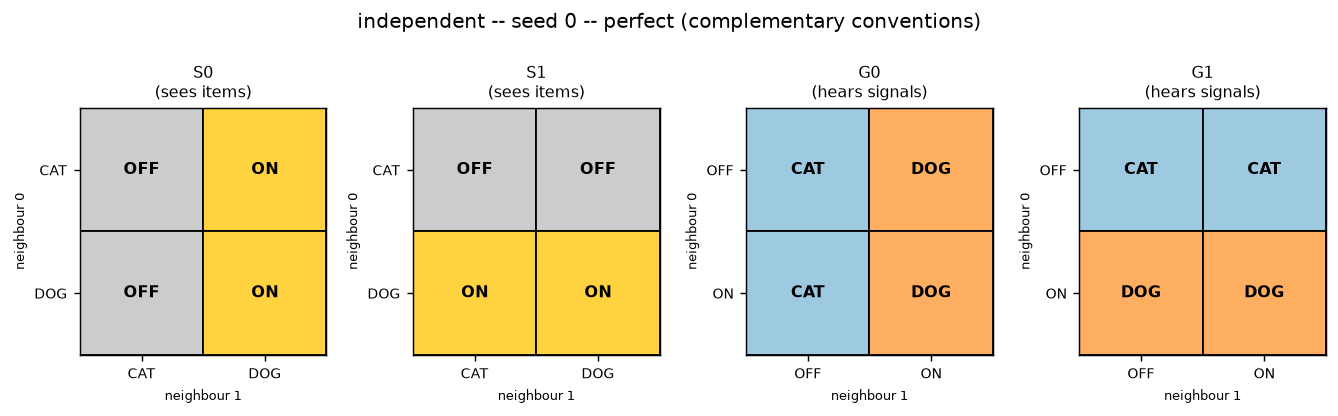
\includegraphics[width=0.47\linewidth]{images/results/k22/conventions_independent_seed0.png}\hfill
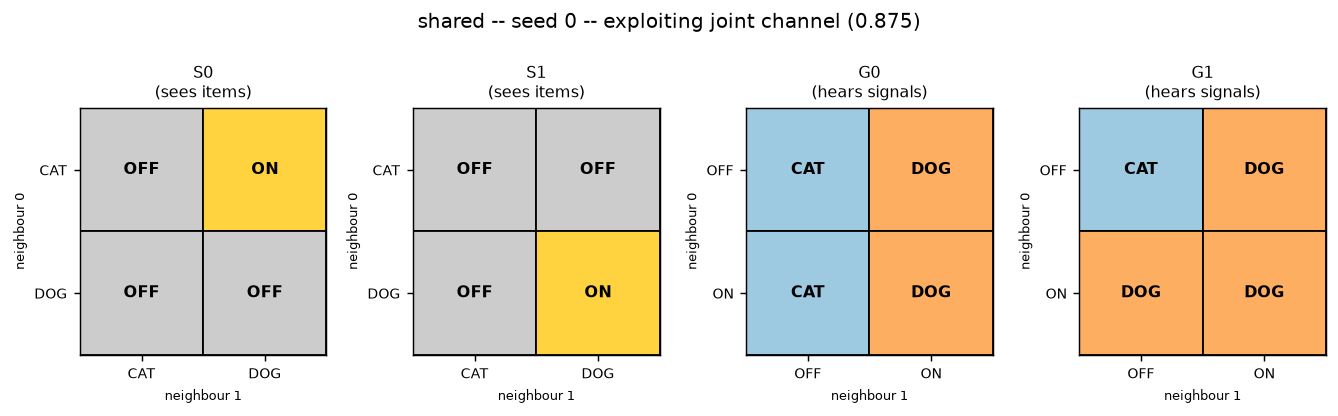
\includegraphics[width=0.47\linewidth]{images/results/k22/conventions_shared_seed0.png}
\caption{Exhaustive greedy-policy heatmaps, $K_{2,2}$, seed 0. Left:
independent-brain variant. Right: shared-brain variant. Each panel is one
agent's complete policy over all four possible observations of its role.}
\label{fig:q1-conventions}
\end{figure}

\subsection{Empirical Action-Response Matrices: Settled Policy}
\label{sec:results-arm-settled}

The exhaustive view above assumes the policy is a clean deterministic
function of its input, which is exactly true of a fully converged greedy
agent but not of a genuinely stochastic one. The complementary tool plays a
batch of $1{,}000$ real episodes with exploration forced off and, for every
$(S_i, G_j)$ edge in the graph, tallies how often each (emitted signal,
produced guess) pair actually occurred
(\texttt{all\_edges\_action\_response\_frequencies}). This was run for the
oracle, the random baseline, and all three trained variants on $K_{2,2}$
(Figure~\ref{fig:q1-arm-settled}).

\begin{figure}[H]
\centering
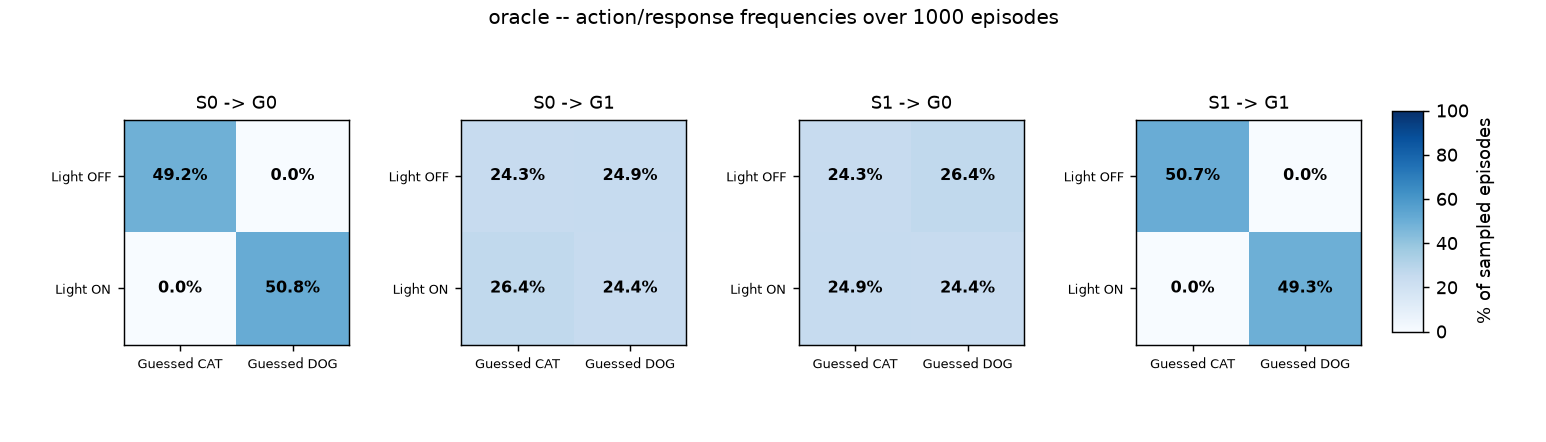
\includegraphics[width=0.32\linewidth]{images/results/k22/action_response_oracle.png}\hfill
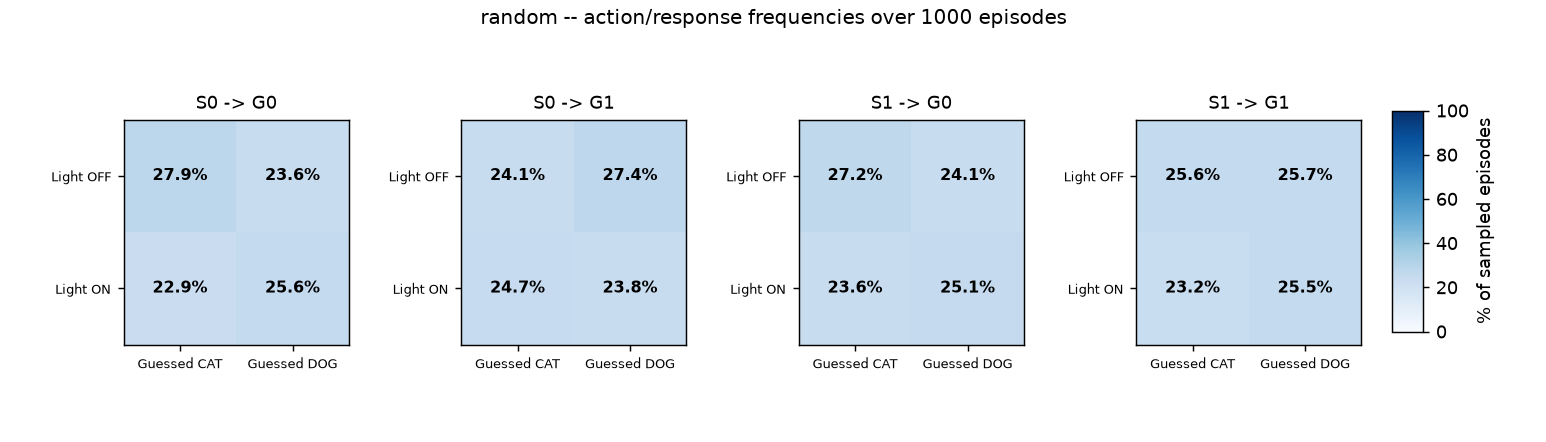
\includegraphics[width=0.32\linewidth]{images/results/k22/action_response_random.png}\hfill
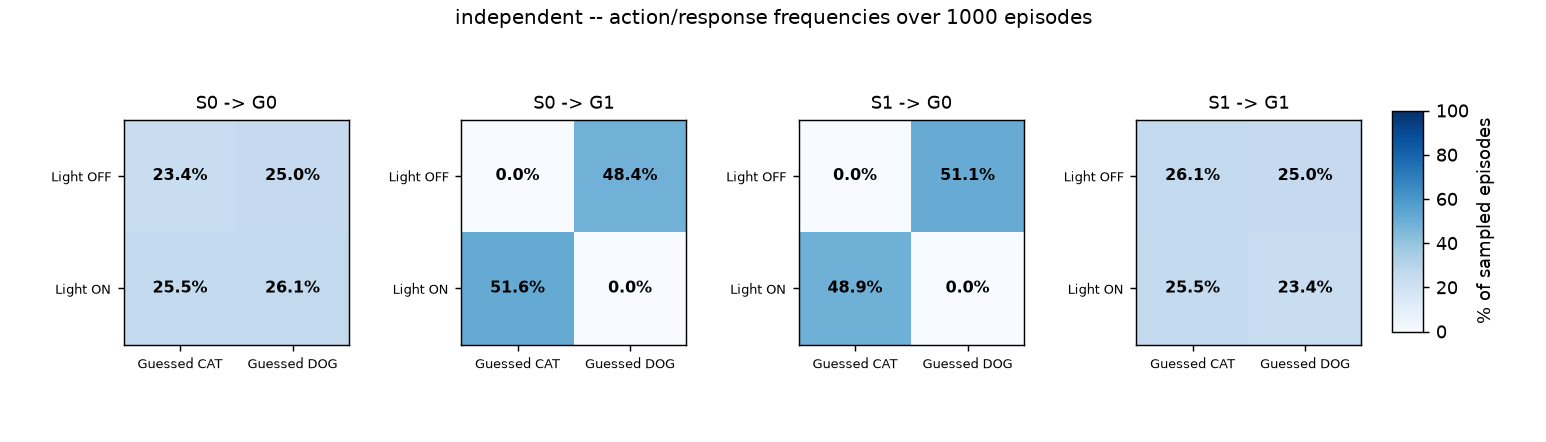
\includegraphics[width=0.32\linewidth]{images/results/k22/action_response_independent.png}
\caption{Empirical action-response matrices, $K_{2,2}$, 1{,}000 greedy
episodes. Left: oracle. Centre: random baseline. Right: independent-brain
variant. Rows are the signaller's emitted signal (Light OFF/ON); columns are
the guesser's produced guess (CAT/DOG); cell colour and percentage are the
empirical joint frequency over the sampled episodes.}
\label{fig:q1-arm-settled}
\end{figure}

The qualitative pattern established here recurs throughout: on $K_{2,2}$, the
oracle and every trained variant that reaches a working convention
concentrates each edge's probability mass onto two of the four cells (a clear
diagonal-like or anti-diagonal-like pattern), while the random baseline
stays close to a flat 25\% in every cell of every edge, exactly as predicted
(Section~\ref{sec:baseline-floor}) for a policy with no rule to have gotten
lucky about. A further, consistent structural finding across the oracle and
every trained variant is that only \emph{two} of the graph's four edges are
``load-bearing'' (carrying a genuine, concentrated signal-guess correlation)
at settled convergence; the other two are structurally present but carry no
more information than the random baseline would produce on them. Which
specific pair of edges ends up load-bearing (i.e.\ which signaller ends up
tracking which guesser) differs from run to run and is, as expected, an
arbitrary but consistent choice within a given run --- precisely the
signature of an implicitly emergent, rather than pre-specified, convention
(Section~\ref{sec:signalling-theory}).

\subsection{Action-Response Matrices During Training}
\label{sec:results-arm-training}

Both tools above characterise the \emph{settled} policy. To see the
convention emerge, rather than only its end state, the same tally
(\texttt{ActionResponseTally}) was instead fed episodes from inside the
training loop itself, with exploration left \emph{on} at whatever epsilon the
schedule currently specifies --- this is what makes the comparison against
the (also-stochastic) random baseline meaningful, rather than comparing a
settled greedy agent against a baseline that never stops exploring. A single
3{,}000-episode training run (seed 0, epsilon linearly decayed to $0.05$ over
1{,}800 episodes) was divided into four disjoint 750-episode windows, and the
tally was reset at each window boundary.

\begin{table}[H]
\centering
\caption{Per-edge peak action-response cell (\% of episodes in that window),
$K_{2,2}$, exploration on. Window~0 = episodes 0--749 ($\epsilon:
1.00\!\to\!0.60$); Window~3 = episodes 2250--2999 ($\epsilon = 0.05$,
converged).}
\label{tab:q1-arm-windowed}
\renewcommand{\arraystretch}{1.2}
\begin{tabular}{l l cccc}
\toprule
\textbf{Variant} & \textbf{Window} & $S_0\!\to\!G_0$ & $S_0\!\to\!G_1$ & $S_1\!\to\!G_0$ & $S_1\!\to\!G_1$ \\
\midrule
\multirow{2}{*}{Random}      & 0 & 27\% & 25\% & 27\% & 25\% \\
                              & 3 & 27\% & 27\% & 27\% & 29\% \\
\multirow{2}{*}{Shared}      & 0 & 27\% & 28\% & 26\% & 31\% \\
                              & 3 & \textbf{50\%} & 26\% & 26\% & \textbf{49\%} \\
\multirow{2}{*}{Two-brain}   & 0 & 31\% & 32\% & 31\% & 32\% \\
                              & 3 & \textbf{53\%} & \textbf{54\%} & \textbf{48\%} & \textbf{48\%} \\
\multirow{2}{*}{Independent} & 0 & 26\% & 31\% & 32\% & 30\% \\
                              & 3 & 26\% & \textbf{51\%} & \textbf{50\%} & 27\% \\
\bottomrule
\end{tabular}
\end{table}

Three findings stand out. First, in Window~0 every variant, trained or not,
looks statistically indistinguishable from the random baseline (all cells in
the high-20s to low-30s percent range) --- with epsilon near 1.0 the agents
are almost entirely exploring, so no convention has had a chance to express
itself yet. Second, by Window~3 (post-decay), the random baseline is
unchanged from Window~0, while every trained variant has developed sharp,
non-uniform structure, directly visualising the "flat $\to$ structured"
transition as epsilon decays. Third, and most interesting: shared-brain and
independent both settle into the same \emph{two-load-bearing-edge} structure
identified in Section~\ref{sec:results-arm-settled} (note the two boldfaced
cells per variant, on different edge pairs for each --- shared happens to
load-bear on the two same-index edges $S_0\!\to\!G_0$/$S_1\!\to\!G_1$ in this
particular run, independent on the cross edges $S_0\!\to\!G_1$/$S_1\!\to\!G_0$),
but \emph{two-brain saturates all four edges simultaneously} (48--54\%
across the board). This is consistent with two-brain's higher mean reward in
Table~\ref{tab:q1-variant-comparison}: sharing parameters within a role, but
not across roles, appears to let both signallers' shared network arrive at a
policy where every edge carries genuine information, rather than settling for
a sparser two-edge convention.

\subsection{Cumulative vs.\ Disjoint Windows: A Dilution Effect}
\label{sec:results-arm-cumulative}

A natural question is whether the windowed tallies above are cumulative
(each window folding in everything before it) or genuinely disjoint. They are
disjoint by construction, and the difference matters empirically: the same
independent-variant run was re-analysed with the tally left running
\emph{cumulatively} across four checkpoints (episodes $0$--$749$,
$0$--$1499$, $0$--$2249$, and $0$--$2999$) rather than reset at each window.

\begin{table}[H]
\centering
\caption{Independent variant, $K_{2,2}$: peak cell on the load-bearing edges,
cumulative tally vs.\ the disjoint final window (both from the same training
run, seed 0).}
\label{tab:q1-arm-cumulative}
\begin{tabular}{lcc}
\toprule
\textbf{Measurement} & $S_0\!\to\!G_1$ & $S_1\!\to\!G_0$ \\
\midrule
Cumulative, episodes 0--749   & 31\% & 32\% \\
Cumulative, episodes 0--1499  & 36\% & 35\% \\
Cumulative, episodes 0--2249  & 41\% & 40\% \\
Cumulative, episodes 0--2999 (full run) & 43\% & 42\% \\
\midrule
Disjoint, final window only (2250--2999) & 51\% & 50\% \\
\bottomrule
\end{tabular}
\end{table}

The cumulative measure at the end of training (42--43\%) noticeably
understates the actual settled behaviour of the final window (50--51\%): a
substantial fraction of the cumulative history is still pure early-training
exploration, and that mass permanently dilutes any statistic computed over
the whole run. This confirms that a windowed, disjoint measurement is the
correct choice for characterising "what has the agent settled into," while a
cumulative measurement instead answers "what has the agent done on average
across its entire training history" --- a different, and for this purpose
less useful, question.

\section{Extending Beyond \texorpdfstring{$K_{2,2}$}{K2,2}: A Preliminary Scaling Probe}
\label{sec:results-scaling}

As a first look toward Question~2's systematic topology analysis
(Section~\ref{sec:q2}), the identical environment, training, and evaluation
pipeline used above (unchanged code, per Section~\ref{sec:results-implementation})
was applied to the ratio-1 complete-bipartite family $K_{m,m}$ for
$m \in \{3,4,5,6\}$. This is explicitly a \emph{preliminary, single-seed}
probe (seed 0 only), not the $P=30$ protocol that Question~2's Family~A
(Section~\ref{sec:topconditions}) will eventually require at these sizes; it
is reported here as an early indication of how the three variants' behaviour
changes with scale, ahead of the formal multi-seed structural-quality study.
Because larger graphs plausibly need a longer schedule to settle, the
training length was scaled with $m$ rather than held fixed, per
Table~\ref{tab:q1-scaling-schedule}.

\begin{table}[H]
\centering
\caption{Training schedule used for the $K_{m,m}$ scaling probe (single seed,
per graph size).}
\label{tab:q1-scaling-schedule}
\begin{tabular}{lcccc}
\toprule
& $K_{3,3}$ & $K_{4,4}$ & $K_{5,5}$ & $K_{6,6}$ \\
\midrule
Training episodes            & 5{,}000 & 7{,}000 & 9{,}000 & 12{,}000 \\
$\epsilon$ decay episodes    & 3{,}200 & 4{,}500 & 6{,}000 & 8{,}000 \\
Live action-response tally   & \multicolumn{4}{c}{every training episode above (exploration on)} \\
Settled greedy evaluation    & \multicolumn{4}{c}{2{,}000 episodes, $\epsilon = 0$, held-out seed} \\
\bottomrule
\end{tabular}
\end{table}

\subsection{Team Reward Across Graph Size}

\begin{table}[H]
\centering
\caption{Settled greedy team reward, $K_{m,m}$ scaling probe, single seed
(0). Convergence bands from Section~\ref{sec:baselines}: $0.50$ floor, $0.75$
single-bit ceiling, $1.00$ oracle ceiling.}
\label{tab:q1-scaling-reward}
\renewcommand{\arraystretch}{1.25}
\begin{tabular}{lcccc}
\toprule
\textbf{Variant} & $K_{3,3}$ & $K_{4,4}$ & $K_{5,5}$ & $K_{6,6}$ \\
\midrule
Random       & 0.506 & 0.493 & 0.502 & 0.495 \\
Shared-brain & 0.831 & 0.780 & 0.758 & \textbf{0.846} \\
Two-brain    & \textbf{0.918} & \textbf{0.892} & 0.839 & 0.811 \\
Independent  & 0.878 & 0.862 & \textbf{0.853} & 0.833 \\
\bottomrule
\end{tabular}
\end{table}

Every trained variant clears the random floor by a wide margin at every
graph size, and every variant sits in the "single-bit ceiling / exploiting
joint channel" band ($0.75$--$0.95$) rather than reaching the theoretical
$1.00$ ceiling (Section~\ref{sec:results-baselines}) at any size beyond
$K_{2,2}$. Two-brain leads at the two smallest sizes ($K_{3,3}$, $K_{4,4}$),
but declines monotonically as $m$ grows (0.918 $\to$ 0.892 $\to$ 0.839 $\to$
0.811); independent stays comparatively flat and overtakes two-brain at
$K_{5,5}$; and shared-brain, after declining from $K_{3,3}$ to $K_{5,5}$,
reverses and \emph{increases} at $K_{6,6}$ (0.758 $\to$ 0.846), briefly
exceeding two-brain for the first time in the sweep. With only a single seed
per condition these particular crossovers should be read as suggestive
rather than conclusive --- they are exactly the kind of question the planned
$P=30$ protocol at each size (Question~2) is designed to settle definitively.

\subsection{Live Action-Response Matrices: Methodology}
\label{sec:results-scaling-methodology}

The first version of this scaling probe measured each population's
action-response matrix the same way Section~\ref{sec:results-arm-settled}
does at $K_{2,2}$: freeze the trained policy greedy ($\epsilon=0$) and play a
fresh batch of episodes. That approach was replaced with the \emph{live}
methodology of Section~\ref{sec:results-arm-training}, extended here across
all four graph sizes: the tally is fed from the training episodes themselves,
exploration \emph{on}, epsilon decaying on its normal schedule, rather than
from a separate frozen-deterministic pass. The random baseline is played for
exactly the same number of episodes as that size's training schedule
(Table~\ref{tab:q1-scaling-schedule}), so a variant that is still learning is
compared against a baseline over an identical episode budget --- an
apples-to-apples comparison that a frozen-greedy trained policy versus an
always-stochastic random policy does not give. The settled greedy team reward
in Table~\ref{tab:q1-scaling-reward} is still measured separately, on a
held-out $2{,}000$-episode greedy pass, and is independent of the live tally.

Because the live tally spans the \emph{entire} training run --- most of which
happens before $\epsilon$ has decayed very far --- every percentage reported
below is diluted toward $25\%$ by early, near-uniformly-random episodes, in
exactly the way Section~\ref{sec:results-arm-cumulative}'s cumulative-vs-disjoint
comparison quantified at $K_{2,2}$. A peak cell of $60$--$75\%$ here should
therefore be read as \emph{"this edge has a real, directional rule"}, not as
\emph{"this edge is only 60--75\% reliable"}; the settled greedy reward in
Table~\ref{tab:q1-scaling-reward} is the trustworthy accuracy figure, and is
consistently higher than what the raw peak percentages alone would suggest.

\begin{figure}[H]
\centering
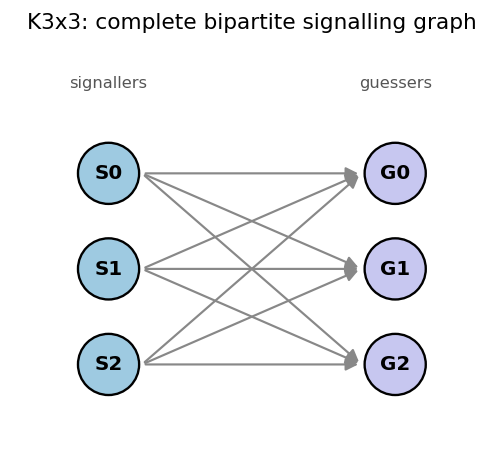
\includegraphics[width=0.23\linewidth]{images/results/k3x3/graph_topology.png}\hfill

\includegraphics[width=0.23\linewidth]{images/results/k4x4/graph_topology.png}\hfill

\includegraphics[width=0.23\linewidth]{images/results/k5x5/graph_topology.png}\hfill

\includegraphics[width=0.23\linewidth]{images/results/k6x6/graph_topology.png}
\caption{The four complete-bipartite graphs of the scaling probe, $K_{3,3}$
through $K_{6,6}$ (left to right).}
\label{fig:q1-scaling-topologies}
\end{figure}

As with random at $K_{2,2}$, the random baseline stays flat at $\approx 25\%$
in every cell of every edge at every graph size probed here, with no
exceptions --- confirming that no spurious structure emerges from grid size
alone, and that everything reported below for the trained variants is real.

\subsection{Convention Patterns by Graph Size}
\label{sec:results-scaling-patterns}

\paragraph{$K_{3,3}$ (two-brain, $R=0.918$).} Rather than the "obvious"
diagonal pairing ($S_i$ serving $G_i$), two-brain settles on a clean
\emph{3-cycle}: $S_0\!\to\!G_1$ (OFF$\to$CAT, ON$\to$DOG), $S_1\!\to\!G_2$
(OFF$\to$DOG, ON$\to$CAT), and $S_2\!\to\!G_0$ (OFF$\to$CAT, ON$\to$DOG) are
all sharply directional (70--81\% of mass on the two "correct" cells), while
the remaining six of the nine edges are flat. This generalises $K_{2,2}$'s
"exactly two load-bearing edges out of four" finding
(Section~\ref{sec:results-arm-settled}) to "exactly $m$ load-bearing edges
out of $m^2$, forming a bijection between signallers and guessers" ---
except the bijection found here is a permutation, not the identity.

\begin{figure}[H]
\centering
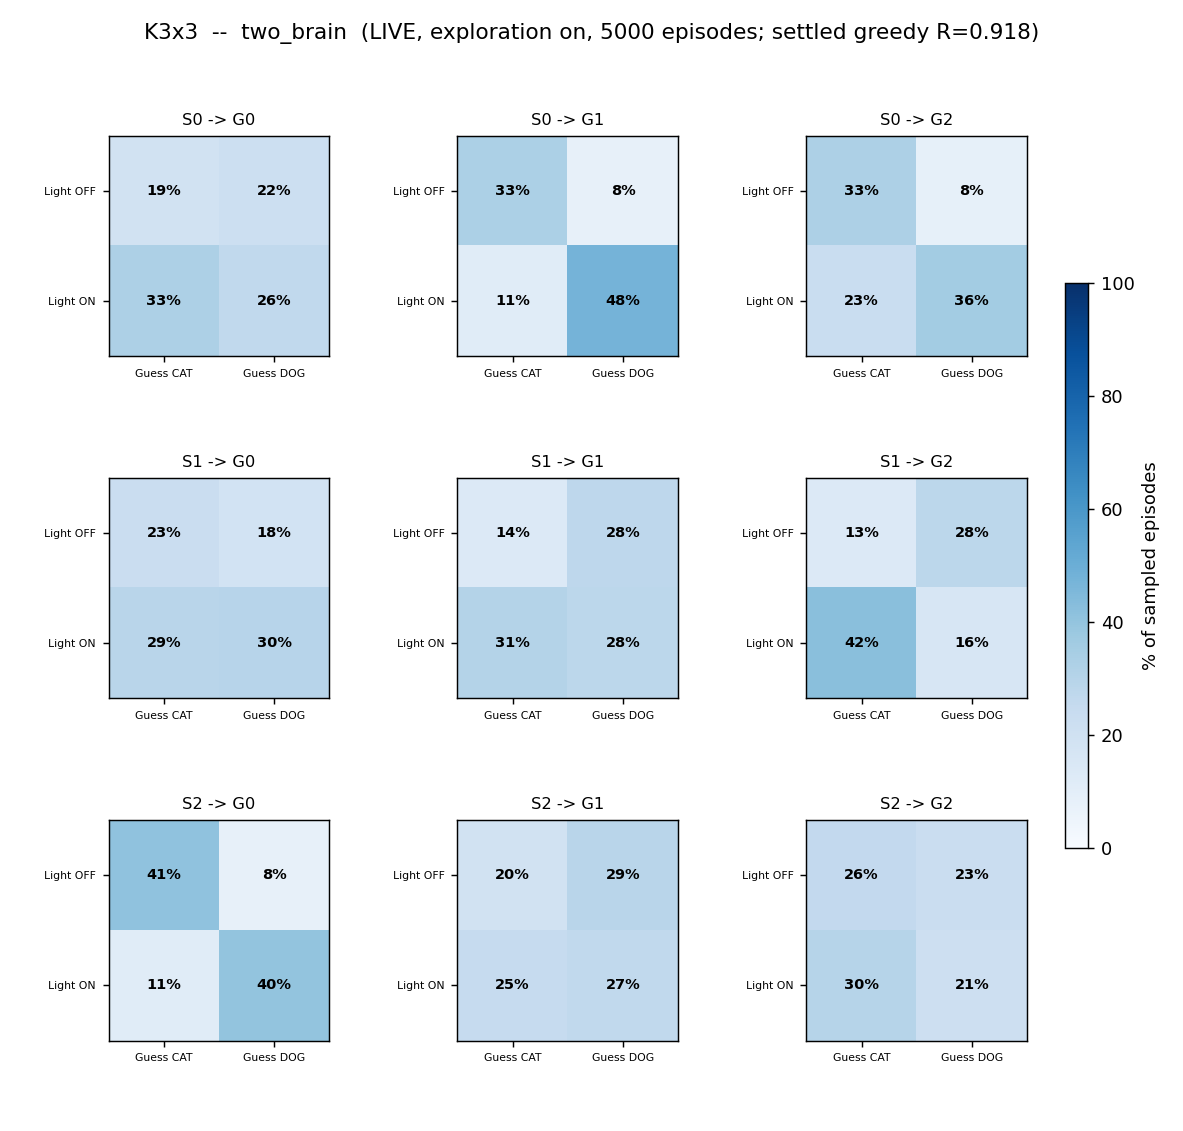
\includegraphics[width=0.62\linewidth]{images/results/k3x3/action_response_two_brain.png}
\caption{$K_{3,3}$, two-brain variant, live action-response matrix
(exploration on, 5{,}000 episodes). The three boldfaced-in-text edges
$S_0\!\to\!G_1$, $S_1\!\to\!G_2$, $S_2\!\to\!G_0$ form a clean 3-cycle; the
other six edges are flat.}
\label{fig:q1-arm-k33}
\end{figure}

\paragraph{$K_{4,4}$ (shared-brain, $R=0.780$).} Because shared-brain is
literally one network evaluated at every node, the same rule
(OFF$\to$DOG, ON$\to$CAT) generalises across signaller identities: nearly
every $S_i\!\to\!G_j$ edge for $j \in \{0,1,3\}$ shows this pattern. $G_2$ is
the exception --- every edge into $G_2$, from every signaller, is flat and
CAT-biased regardless of the incoming signal, i.e.\ $G_2$ has defaulted to a
majority-vote guess rather than decoding. Three well-served guessers and one
guesser that failed to decode at all is consistent with a settled reward
just below the earlier sizes.

\begin{figure}[H]
\centering
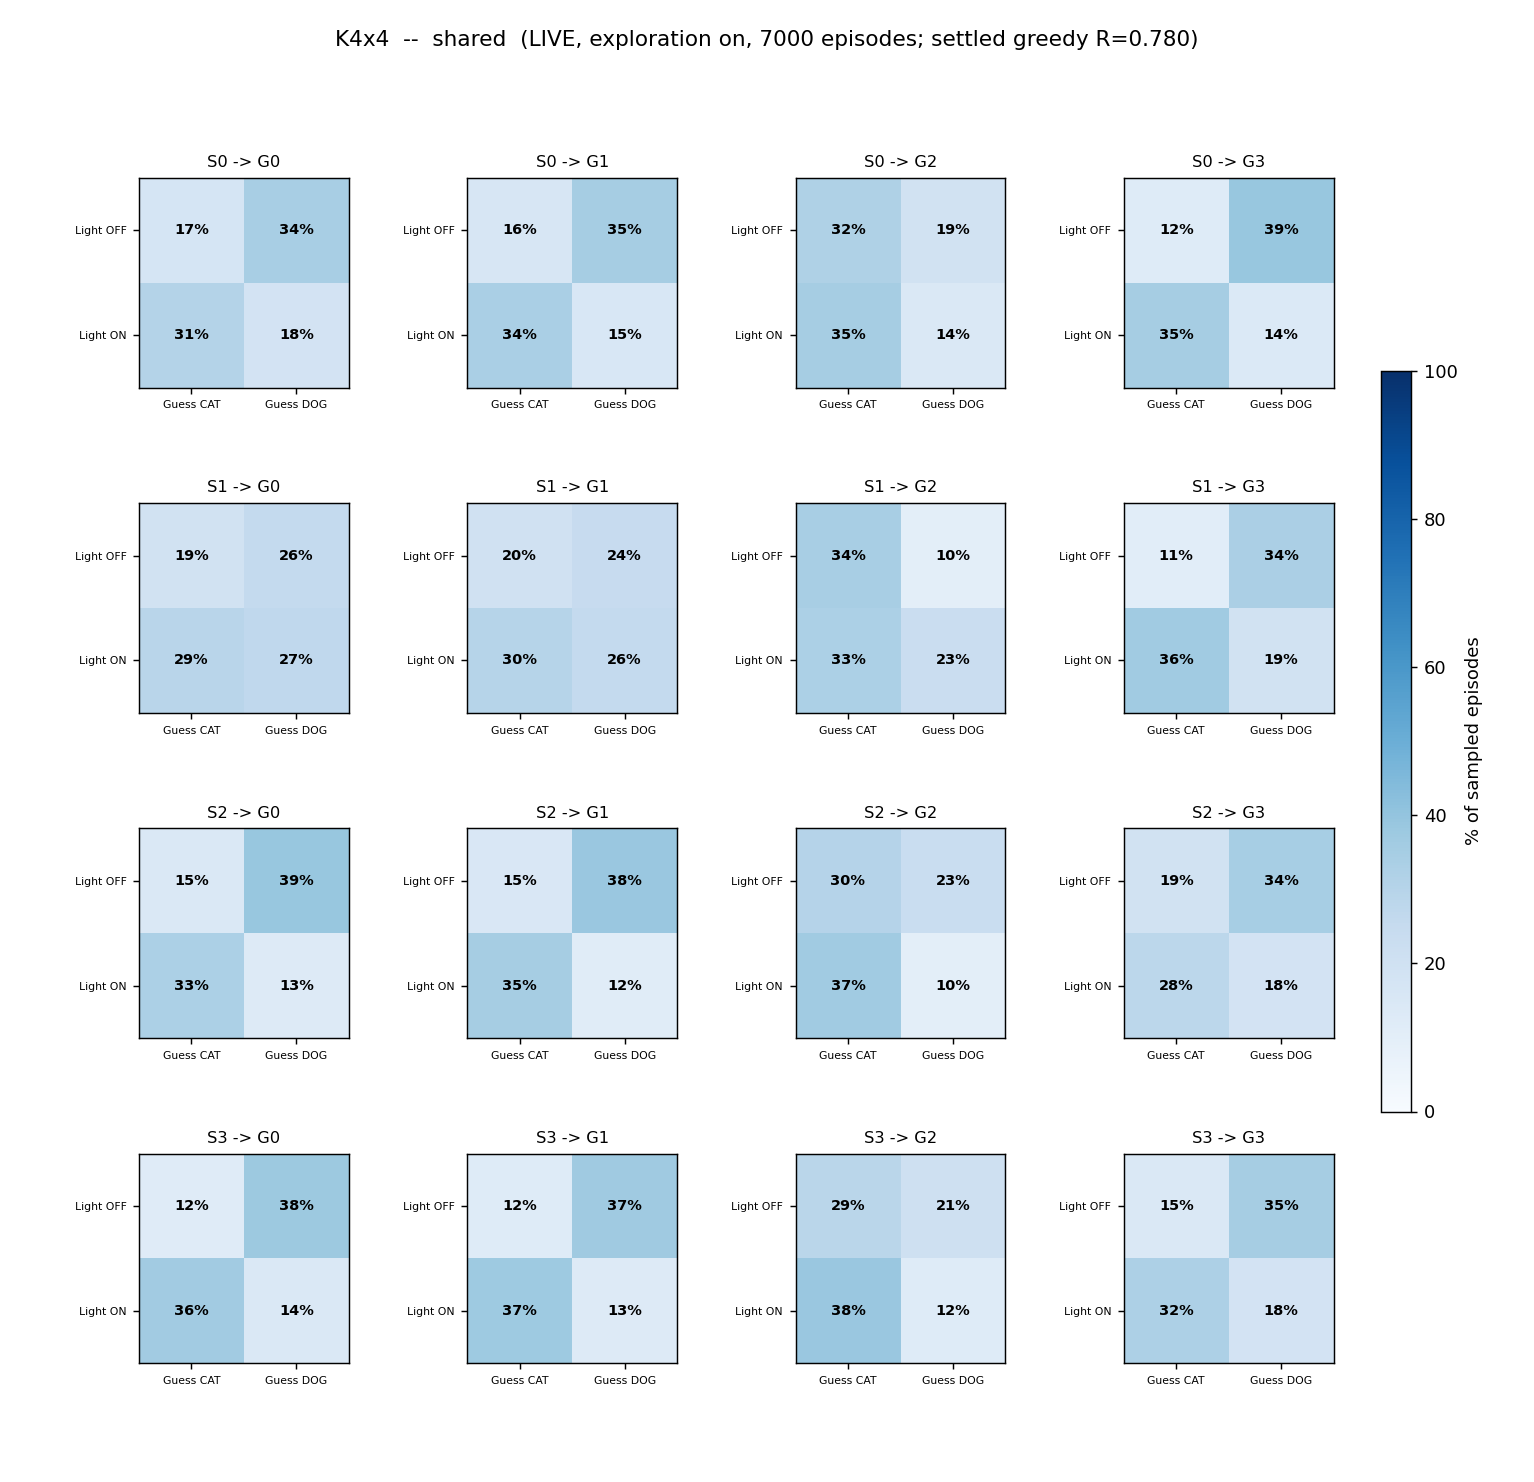
\includegraphics[width=0.75\linewidth]{images/results/k4x4/action_response_shared.png}
\caption{$K_{4,4}$, shared-brain variant, live action-response matrix
(exploration on, 7{,}000 episodes). Columns $S_*\!\to\!G_0$, $G_1$, $G_3$
show the same OFF$\to$DOG/ON$\to$CAT rule from every signaller; column
$S_*\!\to\!G_2$ is flat throughout --- $G_2$ never learned to decode.}
\label{fig:q1-arm-k44}
\end{figure}

\paragraph{$K_{5,5}$ (shared-brain, $R=0.758$).} Here the single shared
network splits into \emph{two} distinct, opposite-direction conventions
rather than one global rule: $G_2$, $G_3$, $G_4$ are served (moderately
cleanly) by "OFF$\to$DOG, ON$\to$CAT" from several signallers, while $G_0$ is
served by $S_3$ and $S_4$ with the \emph{opposite} rule, "OFF$\to$CAT,
ON$\to$DOG". $G_1$, once again, is flat and CAT-biased from every incoming
edge --- the same failure-to-decode pattern seen for $G_2$ at $K_{4,4}$.

\begin{figure}[H]
\centering

\includegraphics[width=0.85\linewidth]{images/results/k5x5/action_response_shared.png}
\caption{$K_{5,5}$, shared-brain variant, live action-response matrix
(exploration on, 9{,}000 episodes). $G_0$ is served by $S_3$/$S_4$ with one
convention direction; $G_2$--$G_4$ are served by the opposite direction from
several other signallers; $G_1$ is flat throughout.}
\label{fig:q1-arm-k55}
\end{figure}

\paragraph{$K_{6,6}$ (independent, $R=0.833$).} At the largest size probed,
no edge reaches the sharpness seen at $K_{3,3}$: peaks are mostly in the
$30$--$38\%$ range rather than $K_{3,3}$'s $70$--$81\%$, and directional
signal is spread thinly across many edges rather than concentrated on a
small dedicated set. This is consistent with the general
increasing-diffuseness-with-$m$ pattern (also visible for shared-brain and
two-brain at $K_{6,6}$, not shown), and --- given the dilution caveat above
--- is most plausibly explained by the fixed single-seed schedule not being
long enough, at this size, for the population to fully settle before the
live tally's episode budget runs out.

\begin{figure}[H]
\centering

\includegraphics[width=0.9\linewidth]{images/results/k6x6/action_response_independent.png}
\caption{$K_{6,6}$, independent variant, live action-response matrix
(exploration on, 12{,}000 episodes). Peaks are visibly more diffuse
(mostly $30$--$38\%$) than at $K_{3,3}$ (Figure~\ref{fig:q1-arm-k33}).}
\label{fig:q1-arm-k66}
\end{figure}

The full battery of figures --- one live action-response matrix per (graph
size, variant) pair, 16 in total, plus the four topology diagrams above ---
is available under \texttt{results/question1/figures/k\{m\}x\{m\}/}, named
\texttt{action\_response\_\{variant\}.png} and \texttt{graph\_topology.png}.

\subsection{Cross-Cutting Patterns: Failing Guessers and Conflicting Edges}
\label{sec:results-scaling-crosscutting}

Two qualitative patterns recur across sizes and variants, beyond the
per-graph descriptions above.

\paragraph{A guesser can fail to decode entirely while others succeed.} This
is a genuine qualitative failure mode, not merely "lower accuracy" on that
guesser: $G_2$ at $K_{4,4}$ (shared-brain) and $G_1$ at $K_{5,5}$
(shared-brain) both show every one of their incoming edges flat and
CAT-biased, i.e.\ the guesser has settled on "always guess CAT" rather than
conditioning on any received signal at all. The same pattern appears for
$G_1$ at $K_{4,4}$ under two-brain, and $G_0$ at $K_{3,3}$ under independent
has no clean incoming edge from any of its three signallers.

\paragraph{Conflicting-direction edges appear where networks are less
shared.} When two signallers independently feeding the same guesser are not
forced to share parameters, they can settle on \emph{opposite} conventions
into that guesser. At $K_{4,4}$ under independent, $S_1\!\to\!G_1$ shows
"OFF$\to$DOG, ON$\to$CAT" while $S_2\!\to\!G_1$ shows the reverse; the same
happens for $S_1\!\to\!G_2$ versus $S_2\!\to\!G_2$ in the same run. This is a
direct, visible consequence of independent training having no mechanism to
force two signallers feeding the same guesser to agree on which direction
means what --- a concrete illustration of the "arbitrary but locally
consistent" character of an implicitly emergent convention
(Section~\ref{sec:signalling-theory}), now visible \emph{within} a single
population rather than only across independently-trained ones.

\subsection{Computational Cost by Variant}

\begin{table}[H]
\centering
\caption{Wall-clock training time (seconds) per (graph, variant), single
run, 8-CPU node.}
\label{tab:q1-scaling-time}
\begin{tabular}{lcccc}
\toprule
\textbf{Variant} & $K_{3,3}$ & $K_{4,4}$ & $K_{5,5}$ & $K_{6,6}$ \\
\midrule
Random       & 0.0  & 0.0  & 0.1  & 0.1 \\
Shared-brain & 24.1 & 12.0 & 16.9 & 24.7 \\
Two-brain    & 12.3 & 18.0 & 24.4 & 34.6 \\
Independent  & 31.3 & 58.6 & 96.7 & 156.0 \\
\bottomrule
\end{tabular}
\end{table}

This is the clearest confirmation of the architectural difference described
in Section~\ref{sec:rl}: shared-brain and two-brain train exactly one or two
networks regardless of graph size, so their training cost stays roughly flat
as $m$ grows (12--35s across the whole sweep), while independent instantiates
one network \emph{per agent} and its cost grows accordingly --- from 31.3s at
$K_{3,3}$ (6 agents) to 156.0s at $K_{6,6}$ (12 agents), a 5$\times$ increase
for a 2$\times$ increase in agent count. (These timings predate the
switch to the live action-response methodology of
Section~\ref{sec:results-scaling-methodology}; the live tally adds only a
lightweight per-episode bookkeeping cost on top of the same underlying
network-count-driven scaling, so the qualitative pattern is unaffected.) The
entire sweep (4 graph sizes $\times$ 4 variants, including topology and
action-response figure generation) completed in under ten minutes of
wall-clock time on the cluster, indicating that both substantially larger
$K_{m,m}$ graphs and the full $P=30$ protocol at these sizes remain
comfortably tractable.

\section{Outstanding Work for Question 1}
\label{sec:q1-outstanding}

The following items from Section~\ref{sec:eval-criteria} and
Section~\ref{sec:baselines} are implemented in structure but not yet run, or
not yet implemented at all, and are the immediate next steps before Question~1
can be considered complete:

\begin{itemize}
    \item \textbf{Information-theoretic metrics}: mutual information
    $I(M_i; x_j)$ per signaller--guesser pair, channel utilisation
    $H(M_i)/1$, and entropy reduction $I(o_j; x_j)$ per guesser, computed over
    the final training window of each of the $P=30$ $K_{2,2}$ runs.
    \item \textbf{Convention-quality metrics}: the joint canonical convention
    distribution $\hat{p}(C_i, C_j)$ across the 30 seeds per variant, the
    complementarity rate, and convention entropy $H$ --- the direct O1.4
    consistency analysis, for which the raw per-seed convention data already
    exists (Section~\ref{sec:results-conventions}) but has not yet been
    aggregated across the full $P=30$ batch.
    \item \textbf{Cross-play evaluation} (Section~\ref{sec:baseline-crossplay}):
    pairing signallers from one of the 30 trained populations with guessers
    from another, to compute the cross-play gap $\Delta$ and test convention
    shareability.
    \item \textbf{No-communication and noisy-channel baselines}
    (Sections~\ref{sec:baseline-nocomm}, \ref{sec:baseline-noisy}): structural
    stubs exist but have not been executed against the trained populations.
    \item \textbf{A general $K_{m,m}$ oracle}, generalising
    \texttt{k22\_oracle} beyond the hand-coded $K_{2,2}$ and matching-graph
    cases, so the scaling probe in Section~\ref{sec:results-scaling} can be
    read against a computed ceiling rather than only against the random floor.
    \item \textbf{The ternary extended-game variant} (Section~\ref{sec:extended-game})
    has not yet been run.
\end{itemize}
    
    
    
    
    % ─── CONCLUSION ──────────────────────────────────────────────────────────────
    \chapter{Conclusion}
    \label{chap:conclusion}
    
    
    \nocite{*}
    
    \bibliography{references}\addcontentsline{toc}{chapter}{References}
    \end{document}
    